\specialchapter{To the reader}

\begin{enumerate}
\def\labelenumi{\arabic{enumi}.}
\item
  The Elements of Mathematics series takes up mathematics at their beginning, and gives complete proofs. In principle, it requires no particular knowledge of mathematics on the reader's part, but only a certain familiarity with mathematical reasoning and a certain capacity for abstract thought. Nevertheless, it is directed especially to those who have a good knowledge of at least the content of the first year or two of a university mathematics course.
\item
  The method of exposition we have chosen is axiomatic, and normally proceeds from the general to the particular. The demands of proof impose a rigorously fixed order on the subject matter. It follows that the utility of certain considerations will not be immediately apparent to the reader unless he already has a fairly extensive knowledge of mathematics.
\item
  The series is divided into Books, and each Book into chapters. The Books already published, either in whole or in part, in the French edition, are listed below. When an English translation is available, the corresponding English title is mentioned between parentheses. Throughout the volume a reference indicates the English edition, when available, and the French edition otherwise.
\end{enumerate}

Théorie des Ensembles (Theory of Sets) designated by E (S)

Algèbre (Algebra) --- A (A)

Topologie Générale (General Topology) --- TG (GT)

(Functions of a Real Variable) --- FVR (FRV)

Espaces Vectoriels Topologiques (Topological Vector Spaces) --- EVT (TVS)

Intégration (Integration) --- INT (INT)

Algèbre Commutative (Commutative Algebra) --- AC (CA)

Variétés Différentielles et Analytiques --- VAR

(Lie Groups and Lie Algebras) --- LIE (LIE)

Théories Spectrales --- TS

In the first six Books (according to the above order), every statement in the text assumes as known only those results which have already been discussed in the same chapter, or in the previous chapters ordered as follows: S; A, Chapters I to III; GT, Chapters I to III; A, from Chapter IV on; GT, from Chapter IV on; FRV; TVS; INT.

From the seventh Book onward, the reader will usually find a precise indication of its logical relationship to the other Books (the first six Books being always assumed to be known).

\begin{enumerate}
\def\labelenumi{\arabic{enumi}.}
\setcounter{enumi}{3}
\item
  However we have sometimes inserted examples in the text that refer to facts the reader may already know but which have not yet been discussed in the series. Such examples are placed between two asterisks: *\ldots*. Most readers will undoubtedly find that these examples help them to understand the text. In other cases, the passages between *\ldots* refer to results that are discussed elsewhere in the series. We hope that the reader will be able to verify the absence of any vicious circle.
\item
  The logical framework of each chapter consists of the definitions, the axioms, and the theorems of the chapter. These are the parts that have mainly to be borne in mind for subsequent use. Less important results and those which can easily be deduced from the theorems are labelled as ``propositions'', ``lemmas'', ``corollaries'', ``remarks'', etc. Those which may be omitted on a first reading are printed in small type. A commentary on a particularly important theorem occasionally appears under the name of ``scholium''.
\end{enumerate}

To avoid tedious repetitions it is sometimes convenient to introduce notations or abbreviations that are in force only within a certain chapter or a certain section of a chapter (for example, in a chapter that is concerned only with commutative rings, the word ``ring'' would always signify ``commutative ring''). Such conventions are always explicitly mentioned, generally at the beginning of the chapter in which they occur.

\pandocbounded{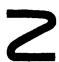
\includegraphics[keepaspectratio]{images/part001_a52dd4e1.jpg}}

\begin{enumerate}
\def\labelenumi{\arabic{enumi}.}
\setcounter{enumi}{5}
\item
  Some passages in the text are designed to forewarn the reader against serious errors. These passages are signposted in the margin with the sign (``dangerous bend'').
\item
  The Exercises are designed both to enable the reader to satisfy himself that he has digested the text and to bring to his attention results that have no place in the text but are nevertheless of interest. The most difficult exercises bear the sign Ⅱ.
\item
  In general, we have adhered to the commonly accepted terminology, except where there appeared to be good reasons for deviating from it.
\item
  We have made a particular effort always to use rigorously correct language, without sacrificing simplicity. As far as possible we have drawn attention in the text to abuses of language, without which any mathematical text runs the risk of pedantry, not to say unreadability.
\item
  Since in principle the text consists of the dogmatic exposition of a theory, it contains in general no references to the literature. Bibliographical references are gathered together in Historical Notes. The bibliography which follows each historical note contains in general only those books and original memoirs that have been of the greatest importance in the evolution of the theory under discussion. It makes no pretense of any sort to completeness.
\end{enumerate}

As to the exercises, we have not thought it worthwhile in general to indicate their origins, since they have been drawn from many different sources (original papers, textbooks, collections of exercises).

\begin{enumerate}
\def\labelenumi{\arabic{enumi}.}
\setcounter{enumi}{10}
\tightlist
\item
  References to a part of this series are given as follows:
\end{enumerate}

\begin{enumerate}
\def\labelenumi{\alph{enumi})}
\item
  If reference is made to theorems, axioms, or definitions presented in the same section (§), they are cited by their number.
\item
  If they occur in another section of the same chapter, this section is also cited in the reference.
\item
  If they occur in another chapter in the same Book, the chapter and section are cited.
\item
  If they occur in another Book, the Book is cited first, by the abbreviation of its title.
\end{enumerate}

The Summaries of Results are cited by the letter R; thus S, R signifies the ``Summary of Results of the Theory of Sets''.

\chapter{Haar measure}

In this chapter and in the next, when we speak of a function (resp. a measure), it will be understood to be either a real or a complex function (resp. measure); if T is a locally compact space, the notation \(\mathcal{K}(T)\) will denote either the space \(\mathcal{K}_{\mathbf{R}}(T)\) or the space \(\mathcal{K}_{\mathbf{C}}(T)\) ; similarly for the notations \(\overline{\mathcal{K}(T)}\) , \(\mathcal{C}(T)\) , \(L^{p}(T,\mu)\) , \(\mathcal{M}(T)\) , etc. It is of course understood that in a situation involving several functions, measures or vector spaces, the results obtained are valid when these functions, measures or vector spaces are all real or all complex. The space \(\overline{\mathcal{K}(T)}\) will always be assumed to be equipped with the topology of uniform convergence, the space \(\mathcal{C}(T)\) with the topology of compact convergence, and the space \(\mathcal{K}(T)\) with the direct limit topology whose definition is reviewed at the beginning of Chapter VI. The notation \(\mathcal{K}_{+}(T)\) will denote the set of functions \(\geqslant0\) of \(\mathcal{K}(T)\) . If \(A\subset T\) , \(\varphi_{A}\) will always denote the characteristic function of A. If \(t\in T\) , \(\varepsilon_{t}\) will denote the positive measure defined by the mass +1 at the point t.

All locally convex spaces will be assumed to be Hausdorff.

We will denote by e the neutral element of all of the groups considered, absent express mention to the contrary.

\section{CONSTRUCTION OF A HAAR MEASURE}

\subsection{Definitions and notations}

Let G be a topological group operating continuously on the left (GT, III, §2, No.~4) in a locally compact space X; for \(s \in G\) and \(x \in X\) , let sx be the transform of x by s. We denote by \(\boldsymbol{\gamma}_{\mathbf{X}}(s)\) , or \(\boldsymbol{\gamma}(s)\) , the homeomorphism of X onto X defined by

\[
\gamma (s) x = s x.\tag{1}
\]

We have

\[
\boldsymbol {\gamma} (s t) = \boldsymbol {\gamma} (s) \boldsymbol {\gamma} (t).\tag{2}
\]

If \(f\) is a function defined on \(X\) , \(\boldsymbol{\gamma}(s)f\) will be defined by transport of structure, that is, by the formula \((\boldsymbol{\gamma}(s)f)(\boldsymbol{\gamma}(s)x) = f(x)\) ; in other words,

\[
\big (\boldsymbol {\gamma} (s) f \big) (x) = f (s ^ {- 1} x).\tag{3}
\]

If \(\mu\) is a measure defined on X, \(\gamma(s)\mu\) will also be defined by transport of structure, which leads to

\[
\langle f, \boldsymbol {\gamma} (s) \mu \rangle = \langle \boldsymbol {\gamma} (s ^ {- 1}) f, \mu \rangle \quad \text {   for   } f \in \mathscr {K} (\mathrm{X}).\tag{4}
\]

In other words,

\[
\int_ {\mathrm{X}} f (x) d (\boldsymbol {\gamma} (s) \mu) (x) = \int_ {\mathrm{X}} f (s x) d \mu (x).\tag{5}
\]

If A is a \((\gamma(s)\mu)\) -integrable set, then \(s^{-1}A\) is \(\mu\) -integrable and

\[
\left(\boldsymbol {\gamma} (s) \mu\right) (\mathrm{A}) = \mu \left(s ^ {- 1} \mathrm{A}\right).\tag{6}
\]

The measure \(\boldsymbol{\gamma}(s)\mu\) may also be defined as the image of \(\mu\) under \(\boldsymbol{\gamma}(s)\) . Instead of writing \(d(\boldsymbol{\gamma}(s)\mu)(x)\) , it is sometimes useful to write \(d\mu(s^{-1}x)\) ; the formula (5) then takes the following form:

\[
\int_ {\mathrm{X}} f (x) d \mu (s ^ {- 1} x) = \int_ {\mathrm{X}} f (s x) d \mu (x);
\]

the expression on the right may then be deduced from that on the left by `replacing \(x\) by \(sx\) .'

DEFINITION 1. --- Let \(\mu\) be a measure on X.

\begin{enumerate}
\def\labelenumi{\alph{enumi})}
\item
  \(\mu\) is said to be invariant under G if \(\pmb{\gamma}(s)\mu = \mu\) for every \(s\in \mathbf{G}\) .
\item
  \(\mu\) is said to be relatively invariant under \(\mathbf{G}\) if \(\pmb{\gamma}(s)\pmb{\mu}\) is proportional to \(\pmb{\mu}\) for every \(s\in \mathbf{G}\) .
\item
  \(\mu\) is said to be quasi-invariant under \(\mathbf{G}\) if \(\pmb{\gamma}(s)\pmb{\mu}\) is equivalent to \(\pmb{\mu}\) for every \(s\in \mathbf{G}\) .
\end{enumerate}

Remarks. --- 1) Assume \(\mu\) invariant. Then \(|\mu|\) , \(\mathcal{R}(\mu)\) , \(\mathcal{I}(\mu)\) are invariant. If \(\mu\) is real, then \(\mu^{+}\) and \(\mu^{-}\) are invariant.

\begin{enumerate}
\def\labelenumi{\arabic{enumi})}
\setcounter{enumi}{1}
\tightlist
\item
  Assume \(\mu\) relatively invariant and nonzero. There exists, for every \(s \in G\) , a unique complex number \(\chi(s)\) such that
\end{enumerate}

\[
\boldsymbol {\gamma} (s) \mu = \chi (s) ^ {- 1} \mu ,\tag{7}
\]

and the function \(\chi\) on \(\mathbf{G}\) is a representation of \(\mathbf{G}\) in \(\mathbf{C}^*\) , called the multiplier of \(\mu\) . The formula (5) then gives

\[
\int_ {\mathrm{X}} f (s x) d \mu (x) = \chi (s) ^ {- 1} \int_ {\mathrm{X}} f (x) d \mu (x),\tag{8}
\]

and formula (6) gives

\[
\mu (s \mathrm{A}) = \chi (s) \mu (\mathrm{A}).\tag{9}
\]

With the conventions made above, (7) may also be written

\[
d \mu (s x) = \chi (s) d \mu (x).\tag{10}
\]

\begin{enumerate}
\def\labelenumi{\arabic{enumi})}
\setcounter{enumi}{2}
\tightlist
\item
  Since \(|\pmb{\gamma}(s)\pmb{\mu}| = \pmb{\gamma}(s)(|\pmb{\mu}|)\) , to say that \(\pmb{\mu}\) is quasi-invariant amounts to saying that \(|\pmb{\mu}|\) is quasi-invariant.
\end{enumerate}

If \(\mu\) is quasi-invariant and \(\mu'\) is another measure on X equivalent to \(\mu\) , then \(\gamma(s)\mu'\) is equivalent to \(\gamma(s)\mu\) , hence to \(\mu\) , hence to \(\mu'\) , and so \(\mu'\) is quasi-invariant. To say that \(\mu\) is quasi-invariant under G therefore means that the class of \(\mu\) is invariant under G.

For \(\mu\) to be quasi-invariant, it is necessary and sufficient that the set of locally \(\mu\) -negligible subsets of X be invariant under G (Ch. V, §5, No.~5, Th. 2), or again that, for every \(\mu\) -negligible compact subset K of X and for every \(s \in \mathbf{G}\) , sK be \(\mu\) -negligible (loc. cit., Remark).

If \(\mu\) is quasi-invariant, then the support of \(\mu\) is invariant under G. In particular if G is transitive in X (A, I, §5, No.~5, Def. 6), this support is either empty (if \(\mu = 0\) ) or equal to X (if \(\mu \neq 0\) ).

Lemma 1. --- Let X, Y, Z be three topological spaces, with Y locally compact. Let \((x,y)\mapsto xy\) be a continuous mapping of \(X\times Y\) into Z, which defines a mapping \(x\mapsto u_{x}\) of X into \(\mathcal{F}(Y;Z)\) by the relation \(u_{x}(y)=xy\) . Let f be a continuous function on Z with values in R or in a Banach space, S the support of f, and \(\mu\) a measure on Y. Assume that for every \(x_{0}\in X\) , there exists a neighborhood V of \(x_{0}\) in X such that \(\bigcup_{x\in V}u_{x}^{-1}(S)\) is relatively compact in Y. Then:

\begin{enumerate}
\def\labelenumi{\alph{enumi})}
\tightlist
\item
  for every \(x \in X\) , \(f \circ u_{x}\) is continuous on Y, with compact support;
\item
  the mapping \(x \mapsto \int_{Y} f(xy) d\mu(y)\) , which is defined by a), is continuous on X.
\end{enumerate}

The assertion a) is obvious. Let us prove b). Since continuity is a local property, we may reduce to the case that \(\bigcup_{x\in X}u_x^{-1}(S)\) is contained in a compact subset \(Y'\) of Y. Since the function \((x,y)\mapsto f(xy)\) is continuous on \(X\times Y\) , \(f\circ u_x\) tends to \(f\circ u_{x_0}\) uniformly on \(Y'\) as \(x\) tends to \(x_0\) (GT, X, §3, No.~4, Th. 3), therefore \(\mu(f \circ u_x)\) tends to \(\mu(f \circ u_{x_0})\) . Whence the lemma.

Let us now return to the previous notations.

PROPOSITION 1. --- Assume that G is locally compact. Let \(\mu\) be a nonzero relatively invariant measure on X. Then its multiplier \(\chi\) is a continuous function on G.

For, let \(f \in \mathcal{K}(\mathbf{X})\) , \(S\) the support of \(f\) , \(s_0\) a point of \(G\) , and \(V\) a compact neighborhood of \(s_0\) in \(G\) ; then, the set

\[
\bigcup_ {s \in V} \gamma (s) ^ {- 1} (S) = V ^ {- 1} S
\]

is compact in X; by Lemma 1 and formula (8), \(\chi(s^{-1})\langle\mu, f\rangle\) depends continuously on \(s\) ; if \(f\) is chosen so that \(\langle\mu, f\rangle \neq 0\) , one sees that \(\chi\) is continuous.

Now let G be a topological group operating continuously on the right in a locally compact space X; for \(s \in G\) and \(x \in X\) , let xs be the transform of x by s. We denote by \(\delta_{\mathbf{X}}(s)\) , or \(\delta(s)\) , the homeomorphism of X defined by

\[
\delta (s) x = x s ^ {- 1}.\tag{1'}
\]

We have

\[
\boldsymbol {\delta} (s t) = \boldsymbol {\delta} (s) \boldsymbol {\delta} (t).\tag{2'}
\]

By transport of structure, one defines the action of \(\boldsymbol{\delta}(s)\) on functions and measures on X:



\[
\big (\boldsymbol {\delta} (s) f \big) (x) = f (x s)\tag{3'}
\]

\[
\langle f, \delta (s) \mu \rangle = \langle \delta (s ^ {- 1}) f, \mu \rangle\tag{4'}
\]

\[
\int_ {\mathrm{X}} f (x) d \bigl (\pmb {\delta} (s) \mu \bigr) (x) = \int_ {\mathrm{X}} f (x s ^ {- 1}) d \mu (x)\tag{5'}
\]

\[
\big (\delta (s) \mu \big) (\mathrm{A}) = \mu (\mathrm{A} s).\tag{6'}
\]

We agree to write \(d\mu(xs)\) in place of \(d(\pmb{\delta}(s)\mu)(x)\) , and \((5')\) then takes the form

\[
\int_ {\mathrm{X}} f (x) d \mu (x s) = \int_ {\mathrm{X}} f (x s ^ {- 1}) d \mu (x).
\]

One defines in an analogous manner the measures on X invariant, relatively invariant and quasi-invariant under G. If \(\mu\) is relatively invariant, its multiplier \(\chi\) is defined by the formulas



\[
\boldsymbol {\delta} (s) \mu = \chi (s) \mu\tag{7'}
\]

\[
\int_ {\mathrm{X}} f (x s) d \mu (x) = \chi (s) ^ {- 1} \int_ {\mathrm{X}} f (x) d \mu (x)\tag{8'}
\]

\[
\mu (\mathrm{A} s) = \chi (s) \mu (\mathrm{A})\tag{9'}
\]

\[
d \mu (x s) = \chi (s) d \mu (x).\tag{10'}
\]

If one regards the group \(G^{0}\) opposite to G as operating in X by \((x, s) \mapsto xs\) , then \(\mu\) is relatively invariant under \(G^{0}\) with the same multiplier \(\chi\) .

Finally, let \(\mathbf{G}\) be a locally compact group. It operates on itself by left and right translations, according to the formulas \(\pmb{\gamma}(s)x = sx\) , \(\pmb{\delta}(s)x = xs^{-1}\) . Then

\[
\boldsymbol {\gamma} (s) \boldsymbol {\delta} (t) = \boldsymbol {\delta} (t) \boldsymbol {\gamma} (s).\tag{11}
\]

All of the foregoing is applicable here, thus we have on G the concepts of measures that are left-invariant, right-invariant, relatively left-invariant, relatively right-invariant, left quasi-invariant, right quasi-invariant (however, see Nos. 8 and 9).

The mapping \(x \mapsto x^{-1}\) is a homeomorphism of \(G\) onto \(G\) . For every function \(f\) on \(G\) , we define the function \(\overset{\vee}{f}\) on \(G\) by

\[
\stackrel {\vee} {f} (x) = f (x ^ {- 1}).\tag{12}
\]

For every measure \(\mu\) on \(\mathbf{G}\) , we define the measure \(\breve{\mu}\) by

\[
\stackrel {\vee} {\mu} (f) = \mu (\stackrel {\vee} {f}) \quad \text { for } f \in \mathcal {K} (\mathrm{G}).\tag{13}
\]

In other words,

\[
\int_ {\mathrm{G}} f (x) d \mu^ {\vee} (x) = \int_ {\mathrm{G}} f (x ^ {- 1}) d \mu (x).\tag{14}
\]

If \(\mathbf{A}\) is a \(\check{\mu}\) -integrable set, then \(\mathbf{A}^{-1}\) is \(\mu\) -integrable and

\[
\check {\mu} (\mathrm{A}) = \mu (\mathrm{A} ^ {- 1}).\tag{15}
\]

We agree to write \(d\mu(x^{-1})\) in place of \(d\check{\mu}(x)\) , and (14) then takes the form

\[
\int_ {\mathrm{G}} f (x) d \mu (x ^ {- 1}) = \int_ {\mathrm{G}} f (x ^ {- 1}) d \mu (x).
\]

\subsection{The existence and uniqueness theorem}

DEFINITION 2. --- Let G be a locally compact group. A nonzero positive measure on G that is left (resp. right) invariant is called a left (resp. right) Haar measure on G.

THEOREM 1. --- On every locally compact group, there exists a left (resp. right) Haar measure, and, up to a constant factor, there exists only one.

\begin{enumerate}
\def\labelenumi{\Alph{enumi})}
\tightlist
\item
  Existence. --- Set \(\mathcal{K}(\mathrm{G}) = \mathcal{K}\) , \(\mathcal{K}_{+}(\mathrm{G}) = \mathcal{K}_{+}\) , \(\mathcal{K}_{+}^{*} = \mathcal{K}_{+} - \{0\}\) . If C is a compact subset of G, we denote by \(\mathcal{K}_{+}^{*}(\mathrm{C})\) the set of \(f \in \mathcal{K}_{+}^{*}\) with support in C. For \(f \in \mathcal{K}\) and \(g \in \mathcal{K}_{+}^{*}\) , there exist numbers \(c_{1}, \ldots, c_{n} \geqslant 0\) and elements \(s_{1}, \ldots, s_{n}\) of G such that \(f \leqslant \sum_{i=1}^{n} c_{i} \gamma(s_{i}) g\) : for, there exists a nonempty open set U in G such that \(\inf_{s \in \mathrm{U}} g(s) > 0\) , and the support of \(f\) can be covered by a finite number of left-translates of U. Let \((f : g)\) be the infimum of the numbers \(\sum_{i=1}^{n} c_{i}\) for all systems \((c_{1}, \ldots, c_{n}, s_{1}, \ldots, s_{n})\) of numbers \(\geqslant 0\) and elements of G such that \(f \leqslant \sum_{i=1}^{n} c_{i} \gamma(s_{i}) g\) . Then:
\end{enumerate}

\begin{enumerate}
\def\labelenumi{(\roman{enumi})}
\item
  \(\left(\pmb{\gamma}(s)f:g\right) = (f:g)\) for \(f\in \mathcal{K}\) , \(g\in \mathcal{K}_{+}^{*}\) , \(s\in G\) ;
\item
  \((\lambda f:g) = \lambda (f:g)\) for \(f\in \mathcal{K}\) \(,g\in \mathcal{K}_{+}^{*},\lambda \geqslant 0\)
\item
  \(\left((f + f^{\prime}):g\right)\leqslant (f:g) + (f^{\prime}:g)\) for \(f\in \mathcal{K},f^{\prime}\in \dot{\mathcal{K}},g\in \mathcal{K}_{+}^{*};\)
\item
  \((f:g)\geqslant (\sup f) / (\sup g)\)
\end{enumerate}

\[
f \in \mathscr {K}, g \in \mathscr {K} _ {+} ^ {*}
\]

\begin{enumerate}
\def\labelenumi{(\alph{enumi})}
\setcounter{enumi}{21}
\tightlist
\item
  \((f:h)\leqslant (f:g)(g:h)\) for \(f\in \mathcal{K}\) \(,g\in \mathcal{K}_{+}^{*}\) \(h\in \mathcal{K}_{+}^{*};\)
\end{enumerate}

\begin{enumerate}
\def\labelenumi{(\roman{enumi})}
\setcounter{enumi}{5}
\item
  \(0 < \frac{1}{(f_0:f)}\leqslant \frac{(f:g)}{(f_0:g)}\leqslant (f:f_0)\) for \(f,f_0,g\) in \(\mathcal{K}_+^*\) ;
\item
  let \(f, f', h\) be in \(\mathcal{K}_+\) with \(h(s) \geqslant 1\) on the support of \(f + f'\) , and let \(\varepsilon > 0\) ; there exists a compact neighborhood \(V\) of \(e\) such that, for every \(g \in \mathcal{K}_+^*(V)\) ,
\end{enumerate}

\[
(f: g) + (f ^ {\prime}: g) \leqslant ((f + f ^ {\prime}): g) + \varepsilon (h: g).
\]

The properties (i), (ii), (iii) are obvious. Let \(f \in \mathcal{K}\) , \(g \in \mathcal{K}_+^*\) ; if \(f \leqslant \sum_{i=1}^{n} c_i \gamma(s_i)g\) with the \(c_i \geqslant 0\) , then \(\sup f \leqslant \sum_{i=1}^{n} c_i g(s_i^{-1}s)\) for some \(s \in \mathbf{G}\) , therefore \(\sup f \leqslant \left( \sum_{i=1}^{n} c_i \right) \sup g\) , whence (iv). Let us now prove (v); let \(f \in \mathcal{K}\) , \(g, h\) in \(\mathcal{K}_+^*\) ; if \(f \leqslant \sum_{i=1}^{n} c_i \boldsymbol{\gamma}(s_i) g\) and \(g \leqslant \sum_{j=1}^{p} d_j \boldsymbol{\gamma}(t_j) h\) ( \(c_i \geqslant 0\) , \(d_j \geqslant 0\) , \(s_i, t_j\) in G), then \(f \leqslant \sum_{i,j} c_i d_j \boldsymbol{\gamma}(s_i t_j) h\) , therefore \((f: h) \leqslant \sum_{i,j} c_i d_j = \left( \sum_{i} c_i \right) \left( \sum_{j} d_j \right)\) ; thus \((f: h) \leqslant (f: g)(g: h)\) . Applying (v) to \(f_0, f, g\) on the one hand and to \(f, f_0, g\) on the other, one obtains (vi). Finally, let \(f, f', h\) be in \(\mathcal{K}_+\) with \(h(s) \geqslant 1\) on the support of \(f + f'\) , and let \(\varepsilon > 0\) . Set \(\mathbf{F} = f + f' + \frac{1}{2} \varepsilon h\) ; the functions \(\varphi, \varphi'\) , that coincide respectively with \(f / F\) and \(f'/F\) on the support of \(f + f'\) and are zero outside it, belong to \(\mathcal{K}_+\) ; for every \(\eta > 0\) , there exists a compact neighborhood V of \(e\) such that \(|\varphi(s) - \varphi(t)| \leqslant \eta\) and \(|\varphi'(s) - \varphi'(t)| \leqslant \eta\) for \(s^{-1} t \in V\) . Then let \(g \in \mathcal{K}_+^*(V)\) ; for every \(s \in G\) ,

\[
\varphi \cdot \boldsymbol {\gamma} (s) g \leqslant (\varphi (s) + \eta) \cdot \boldsymbol {\gamma} (s) g;
\]

for, this is obvious at the points where \(\pmb{\gamma}(s)g\) is zero, therefore outside of \(s\mathbf{V}\) ; and in \(s\mathbf{V}\) , \(\varphi \leqslant \varphi(s) + \eta\) ; similarly, \(\varphi' \cdot \pmb{\gamma}(s)g \leqslant (\varphi'(s) + \eta) \cdot \pmb{\gamma}(s)g\) . This stated, let \(c_1, \ldots, c_n\) be numbers \(\geqslant 0\) and \(s_1, \ldots, s_n\) elements of \(\mathbf{G}\) such that \(\mathbf{F} \leqslant \sum_{i=1}^{n} c_i \pmb{\gamma}(s_i)g\) ; then

\[
f = \varphi \mathrm{F} \leqslant \sum_ {i = 1} ^ {n} c _ {i} \varphi \cdot \boldsymbol {\gamma} (s _ {i}) g \leqslant \sum_ {i = 1} ^ {n} c _ {i} (\varphi (s _ {i}) + \eta) \cdot \boldsymbol {\gamma} (s _ {i}) g
\]

and similarly for \(f'\) ; consequently

\[
(f: g) + (f ^ {\prime}: g) \leqslant \sum_ {i = 1} ^ {n} c _ {i} (\varphi (s _ {i}) + \varphi^ {\prime} (s _ {i}) + 2 \eta) \leqslant (1 + 2 \eta) \sum_ {i = 1} ^ {n} c _ {i}
\]

since \(\varphi +\varphi^{\prime}\leqslant 1\) . Applying the definition of F, then (ii), (iii) and (v), one infers that

\[
\begin{array}{r l} & {(f: g) + (f ^ {\prime}: g) \leqslant (1 + 2 \eta) (\mathrm{F}: g) \leqslant} \\ & {\quad (1 + 2 \eta) \big [ \big ((f + f ^ {\prime}): g \big) + \frac {1}{2} \varepsilon (h: g) \big ] \leqslant} \\ & {\quad \big ((f + f ^ {\prime}): g \big) + \frac {1}{2} \varepsilon (h: g) + 2 \eta \big ((f + f ^ {\prime}): h \big) (h: g) + \varepsilon \eta (h: g)} \end{array}
\]

and, if \(\eta\) has been chosen so that \(\eta\big[2\big((f + f'):h\big) + \varepsilon\big] \leqslant \frac{1}{2}\varepsilon\) , one obtains (vii).

As V runs over the set of compact neighborhoods of \(e\) , the \(\mathcal{K}_{+}^{*}(V)\) form a base of a filter \(\mathfrak{B}\) on \(\mathcal{K}_{+}^{*}\) . Let \(\mathfrak{F}\) be an ultrafilter on \(\mathcal{K}_{+}^{*}\) finer than \(\mathfrak{B}\) . On the other hand, let us fix \(f_{0} \in \mathcal{K}_{+}^{*}\) and let us set, for \(f \in \mathcal{K}_{+}^{*}\) and \(g \in \mathcal{K}_{+}^{*}\) ,

\[
\mathrm{I} _ {g} (f) = \frac {(f : g)}{(f _ {0} : g)}.
\]

By (vi), \(\lim_{g,\mathfrak{F}}\mathrm{I}_g(f) = \mathrm{I}(f)\) exists in the compact space \([1 / (f_0:f),(f:f_0)]\) . By (iii), \(\mathrm{I}(f + f')\leqslant \mathrm{I}(f) + \mathrm{I}(f')\) . By (vii), \(\mathrm{I}(f) + \mathrm{I}(f')\leqslant \mathrm{I}(f + f') + \varepsilon \mathrm{I}(h)\) for all \(\varepsilon >0\) provided \(h\) is \(\geqslant 1\) on the support of \(f + f'\) ; it follows that \(\mathrm{I}(f + f') = \mathrm{I}(f) + \mathrm{I}(f')\) . By Ch. II, §2, No.~1, Prop. 2, I is extendible to a linear form on \(\mathcal{K}\) ; this linear form is a nonzero positive measure on G, left-invariant by (i); this is the sought-for left Haar measure. Passing to the opposite group, one deduces from this the existence of a right Haar measure.

\begin{enumerate}
\def\labelenumi{\Alph{enumi})}
\setcounter{enumi}{1}
\tightlist
\item
  Uniqueness. --- Let \(\mu\) be a left Haar measure, \(\nu\) a right Haar measure. Then \(\check{\nu}\) is a left Haar measure. We are going to show that \(\mu\) and \(\check{\nu}\) are proportional. This will prove that any two left Haar measures are indeed proportional.
\end{enumerate}

Let \(f \in \mathcal{K}\) be such that \(\mu(f) \neq 0\) . By Lemma 1, the function \(D_f\) defined on \(G\) by the formula

\[
\mathrm{D} _ {f} (s) = \mu (f) ^ {- 1} \int f (t ^ {- 1} s) d \nu (t)\tag{16}
\]

is continuous on G. Let \(g \in \mathcal{K}\) . The function \((s, t) \mapsto f(s)g(ts)\) is continuous with compact support in G × G. By Ch. III, §4, No.~1, Th. 2,

\[
\begin{array}{r l} & {\mu (f) \nu (g) = \Big (\int f (s) d \mu (s) \Big) \Big (\int g (t) d \nu (t) \Big)} \\ & {\qquad = \int d \mu (s) \int f (s) g (t s) d \nu (t) = \int d \nu (t) \int f (s) g (t s) d \mu (s)} \\ & {\qquad = \int d \nu (t) \int f (t ^ {- 1} s) g (s) d \mu (s)} \\ & {\qquad = \int g (s) \Big [ \int f (t ^ {- 1} s) d \nu (t) \Big ] d \mu (s) = \mu \big (g \cdot \mu (f) D _ {f} \big),} \end{array}\tag{17}
\]

whence

\[
\nu (g) = \mu (\mathrm{D} _ {f} \cdot g).\tag{18}
\]

This proves, first, that \(D_{f}\) does not depend on f.~For, if \(f' \in H\) is such that \(\mu(f') \neq 0\) , then \(D_{f} \cdot \mu = D_{f'} \cdot \mu\) , therefore \(D_{f} = D_{f'}\) locally almost everywhere for \(\mu\) , hence everywhere, since \(\mathbf{D}_f\) and \(\mathbf{D}_{f'}\) are continuous and the support of \(\mu\) is \(\mathbf{G}\) . We may therefore write \(\mathrm{D}_f = \mathrm{D}\) . The formula (16) gives

\[
\mu (f) \mathrm{D} (e) = \stackrel {\vee} {\nu} (f).\tag{19}
\]

The formula (19) may be extended by linearity to the functions \(f \in \mathcal{K}\) such that \(\mu(f) = 0\) . We have \(D(e) \neq 0\) since \(\check{\nu} \neq 0\) . This indeed establishes the proportionality of \(\mu\) and \(\check{\nu}\) .

COROLLARY. --- Every left-invariant (resp. right-invariant) measure on G is proportional to a left (resp. right) Haar measure.

Examples. --- 1) On the additive group R, the Lebesgue measure dx is a Haar measure (Ch. III, §1, No.~3, Example).

\begin{enumerate}
\def\labelenumi{\arabic{enumi})}
\setcounter{enumi}{1}
\tightlist
\item
  For every function \(f \in \mathcal{K}(\mathbf{R}_+^*)\) , we have (FRV, II, §1, formula (12))
\end{enumerate}

\[
\int_ {0} ^ {+ \infty} \frac {f (x)}{x} d x = \int_ {0} ^ {+ \infty} \frac {f (t x)}{t x} t d x = \int_ {0} ^ {+ \infty} \frac {f (t x)}{x} d x
\]

for all t \textgreater{} 0; the measure \(x^{-1} dx\) is thus a Haar measure on the multiplicative group \(R_{+}^{*}\) .

\begin{enumerate}
\def\labelenumi{\arabic{enumi})}
\setcounter{enumi}{2}
\tightlist
\item
  Let us take for G the torus \(\mathbf{T} = \mathbf{R} / \mathbf{Z}\) . Let \(\varphi\) be the canonical mapping of \(\mathbf{R}\) onto \(\mathbf{T}\) . For \(f \in \mathcal{K}(\mathbf{T})\) , the function \(f \circ \varphi\) is continuous and periodic with period 1 on \(\mathbf{R}\) , and the integral
\end{enumerate}

\[
\mathrm{I} (f) = \int_ {a} ^ {a + 1} f (\varphi (x)) d x
\]

is independent of the choice of \(a \in \mathbf{R}\) ; it is immediate that it is invariant under translation; it therefore defines a Haar measure on \(\mathbf{T}\) . By transport of structure, one deduces from this that \(I(f) = \int_{a}^{a + 1} f(e^{2\pi it}) dt\) is a Haar measure on the multiplicative group \(\mathbf{U}\) of complex numbers of absolute value 1 (GT, VIII, §2, No.~1).

PROPOSITION 2. --- Let G be a locally compact group, \(\mu\) a left or right Haar measure on G. For G to be discrete, it is necessary and sufficient that \(\mu(\{e\}) > 0\) . For G to be compact, it is necessary and sufficient that \(\mu^{*}(G) < +\infty\) .

The conditions are obviously necessary. Let us show their sufficiency. Let V be a compact neighborhood of e. If \(\mu(\{e\}) > 0\) , then V is a finite set since \(\mu(V) < +\infty\) ; since G is Hausdorff, it is therefore discrete. Suppose \(\mu^{*}(G)<+\infty\) and \(\mu\) is, for example, left-invariant. Consider the set \(\mathscr{E}\) of finite subsets \(\{s_{1},\ldots,s_{n}\}\) of G such that \(s_{i}V\cap s_{j}V=\varnothing\) for \(i\neq j\) ; then

\[
n \mu (\mathrm{V}) = \mu (s _ {1} \mathrm{V} \cup \dots \cup s _ {n} \mathrm{V}) \leqslant \mu^ {*} (\mathrm{G}),
\]

therefore \(n \leqslant \mu^{*}(\mathrm{G})/\mu(\mathrm{V})\) . We may therefore choose in E a maximal element \(\{s_{1},\ldots,s_{n}\}\) . Then, for every \(s \in G\) , there exists an i such that \(sV \cap s_{i}V \neq \varnothing\) , hence such that \(s \in s_{i}VV^{-1}\) . Thus G is the union of the compact sets \(s_{i}VV^{-1}\) , hence is compact.

\subsection{Modulus}

Let \(\mu\) be a left Haar measure on G. For every \(s \in \mathbf{G}\) , \(\pmb{\delta}(s)\mu\) is also left-invariant (No.~1, formula (11)), therefore (Th. 1) there exists a unique number \(\Delta_{\mathbf{G}}(s) > 0\) such that \(\pmb{\delta}(s)\mu = \Delta_{\mathbf{G}}(s)\mu\) . By virtue of Th. 1, the number \(\Delta_{\mathbf{G}}(s)\) is independent of the choice of \(\mu\) .

DEFINITION 3. --- The function \(\Delta_{\mathbf{G}}\) on \(\mathbf{G}\) is called the modulus (or modular function) of \(\mathbf{G}\) . If \(\Delta_{\mathbf{G}} = 1\) , the group \(\mathbf{G}\) is said to be unimodular.

One can also say that \(\mu\) is relatively right-invariant with multiplier \(\Delta_{\mathbf{G}}\) . Thus \(\Delta_{\mathbf{G}}\) is a continuous representation of \(\mathbf{G}\) in \(\mathbf{R}_{+}^{*}\) (No.~1, Prop. 1).

Remark. --- If \(\varphi\) is an isomorphism of \(G\) onto a locally compact group \(G'\) , then \(\Delta_{G'} \circ \varphi = \Delta_G\) . In particular:

\begin{enumerate}
\def\labelenumi{\arabic{enumi})}
\item
  Since \(x \mapsto x^{-1}\) is an isomorphism of \(G\) onto the opposite group \(G^0\) , one has \(\Delta_{G^0} = \Delta_{G}^{-1}\) .
\item
  If \(\varphi\) is an automorphism of \(G\) , then \(\Delta_G \circ \varphi = \Delta_G\) .
\end{enumerate}

Let \(s \in G\) . Then:

\[
\boldsymbol {\delta} (s) \left(\Delta_ {\mathrm{G}} ^ {- 1} \cdot \mu\right) = \left(\boldsymbol {\delta} (s) \Delta_ {\mathrm{G}} ^ {- 1}\right) \cdot \left(\boldsymbol {\delta} (s) \mu\right) = \left(\Delta_ {\mathrm{G}} (s) ^ {- 1} \Delta_ {\mathrm{G}} ^ {- 1}\right) \cdot \left(\Delta_ {\mathrm{G}} (s) \mu\right) = \Delta_ {\mathrm{G}} ^ {- 1} \cdot \mu ,
\]

therefore \(\Delta_{\mathrm{G}}^{-1} \cdot \mu = \mu'\) is a right Haar measure. From this, one deduces that \(\boldsymbol{\gamma}(s)\mu' = (\boldsymbol{\gamma}(s)\Delta_{\mathrm{G}}^{-1}) \cdot \mu = \Delta_{\mathrm{G}}(s)(\Delta_{\mathrm{G}}^{-1} \cdot \mu) = \Delta_{\mathrm{G}}(s)\mu'\) , therefore, for every right Haar measure \(\nu\) , we have \(\boldsymbol{\gamma}(s)\nu = \Delta_{\mathrm{G}}(s)\nu\) . Since \(\breve{\mu}\) is a right Haar measure, \(\breve{\mu} = a\Delta_{\mathrm{G}}^{-1} \cdot \mu\) with a constant \(a > 0\) ; it follows that

\[
\mu = a \big (\Delta_ {\mathrm{G}} ^ {- 1} \cdot \mu \big) ^ {\vee} = a \Delta_ {\mathrm{G}} \cdot \stackrel {\vee} {\mu} = a ^ {2} \mu ,
\]

therefore \(a = 1\) and finally \(\check{\mu} = \Delta_{\mathrm{G}}^{-1}\cdot \mu\) . One sees similarly that \(\check{\nu} = \Delta_{\mathrm{G}}\cdot \nu\) . We therefore have the following results:

Formulary. --- Let G be a locally compact group, \(\Delta\) its modulus, \(\mu\) a left Haar measure, and \(\nu\) a right Haar measure.

\begin{enumerate}
\def\labelenumi{\arabic{enumi})}
\tightlist
\item
  One has
\end{enumerate}

\[
\boldsymbol {\gamma} (s) \mu = \mu \quad \boldsymbol {\delta} (s) \mu = \Delta (s) \mu \quad \check {\mu} = \Delta^ {- 1} \cdot \mu .\tag{20}
\]

If \(f\) is \(\mu\) -integrable on \(G\) , then the left and right translates of \(f\) are \(\mu\) -integrable, and

\[
\begin{array}{l} \int f (s x) d \mu (x) = \int f (x) d \mu (x) \\ \int f (x s) d \mu (x) = \Delta (s) ^ {- 1} \int f (x) d \mu (x). \end{array}\tag{21}
\]

Moreover, \(\stackrel{\vee}{f}\) is integrable for \(\Delta^{-1} \cdot \mu\) and

\[
\int f (x ^ {- 1}) \Delta (x) ^ {- 1} d \mu (x) = \int f (x) d \mu (x).\tag{22}
\]

If A is a \(\mu\) -integrable subset of G, then sA and As are \(\mu\) -integrable and

\[
\mu (s \mathrm{A}) = \mu (\mathrm{A}) \quad \mu (\mathrm{A} s) = \Delta (s) \mu (\mathrm{A}).\tag{23}
\]

\begin{enumerate}
\def\labelenumi{\arabic{enumi})}
\setcounter{enumi}{1}
\tightlist
\item
  One has
\end{enumerate}

\[
\boldsymbol {\delta} (s) \nu = \nu \quad \boldsymbol {\gamma} (s) \nu = \Delta (s) \nu \quad \check {\nu} = \Delta \cdot \nu .\tag{24}
\]

If \(f\) is \(\nu\) -integrable on \(G\) , then the left and right translates of \(f\) are \(\nu\) -integrable and

\[
\begin{array}{l} \int f (x s) d \nu (x) = \int f (x) d \nu (x) \\ \int f (s x) d \nu (x) = \Delta (s) \int f (x) d \nu (x). \end{array}\tag{25}
\]

Moreover, \(\stackrel{\vee}{f}\) is integrable for \(\Delta \cdot \nu\) and

\[
\int f (x ^ {- 1}) \Delta (x) d \nu (x) = \int f (x) d \nu (x).\tag{26}
\]

If A is a \(\nu\) -integrable subset of G, then sA and As are \(\nu\) -integrable and

\[
\nu (\mathrm{A} s) = \nu (\mathrm{A}) \quad \nu (s \mathrm{A}) = \Delta (s) ^ {- 1} \nu (\mathrm{A}).\tag{27}
\]

\begin{enumerate}
\def\labelenumi{\arabic{enumi})}
\setcounter{enumi}{2}
\item
  \(\nu\) is proportional to \(\Delta^{-1} \cdot \mu\) , and \(\mu\) is proportional to \(\Delta \cdot \nu\) .
\item
  Suppose G is unimodular. Let \(\mu\) be a Haar measure on G. Then:
\end{enumerate}

\[
\boldsymbol {\gamma} (s) \mu = \boldsymbol {\delta} (s) \mu = \stackrel {\vee} {\mu} = \mu .\tag{28}
\]

If \(f\) is \(\mu\) -integrable on \(G\) , then the left and right translates of \(f\) are \(\mu\) -integrable, as is \(\overset{\vee}{f}\) , and

\[
\int f (s x) d \mu (x) = \int f (x s) d \mu (x) = \int f (x ^ {- 1}) d \mu (x) = \int f (x) d \mu (x).\tag{29}
\]

If \(\mathbf{A}\) is a \(\mu\) -integrable subset of \(\mathbf{G}\) , then \(s\mathbf{A}\) , \(\mathbf{A}s\) and \(\mathbf{A}^{-1}\) are \(\mu\) -integrable and

\[
\mu (s \mathrm{A}) = \mu (\mathrm{A} s) = \mu (\mathrm{A} ^ {- 1}) = \mu (\mathrm{A}).\tag{30}
\]

The analogous properties hold for the essential integral.

PROPOSITION 3. --- If there exists in G a compact neighborhood V of e invariant under the inner automorphisms, then G is unimodular.

For, let \(\mu\) be a left Haar measure on \(\mathbf{G}\) . For every \(s \in \mathbf{G}\) ,

\[
\mu (\mathrm{V}) = \mu (s ^ {- 1} \mathrm{Vs}) = \Delta_ {\mathrm{G}} (s) \mu (\mathrm{V}),
\]

whence \(\Delta_{\mathbf{G}}(s) = 1\) since \(0 < \mu (\mathrm{V}) < +\infty\)

From this, one deduces immediately:

COROLLARY. --- If G is discrete, or compact, or commutative, then G is unimodular.

This is moreover trivial when G is commutative. Note also that if G is discrete, then the measure on G for which each point has mass 1 is obviously a left and right Haar measure on G, called the normalized Haar measure on G. If G is compact, there exists one and only one Haar measure on G such that \(\mu(G)=1\) ; it is called the normalized Haar measure of G. The preceding two conventions are not in accord when G is both discrete and compact, that is, finite; when we are in this case we shall always explicitly specify what is meant by normalized Haar measure.

\pandocbounded{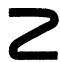
\includegraphics[keepaspectratio]{images/part001_35d0c9a3.jpg}}

Subgroups and quotient groups of a unimodular group are not always unimodular ( \(\S2\) , Exer. 5). See, however, Prop. 10 of \(\S2\) , No.~7.

*We shall see later that semi-simple or nilpotent connected Lie groups are unimodular.*

\subsection{Modulus of an automorphism}

Let G be a locally compact group, \(\varphi\) an automorphism of G, and \(\mu\) a left Haar measure on G. It is clear that \(\varphi^{-1}(\mu)\) is also a left Haar measure on G. Therefore there exists (No.~2, Th. 1) one and only one number a \textgreater{} 0 such that \(\varphi^{-1}(\mu) = a\mu\) . By No.~2, Th. 1, this number is independent of the choice of \(\mu\) . Note that if one had started with a right Haar measure, for example \(\Delta_{G}^{-1} \cdot \mu\) (No.~3), one would have arrived at the same scalar a: for, since \(\varphi^{-1}\) leaves \(\Delta_{G}\) invariant (No.~3, Remark), one has \(\varphi^{-1}(\Delta_{G}^{-1} \cdot \mu) = \Delta_{G}^{-1} \cdot \varphi^{-1}(\mu) = a\Delta_{G}^{-1} \cdot \mu\) .

DEFINITION 4. --- The number a \textgreater{} 0 such that \(\varphi^{-1}(\mu) = a\mu\) is called the modulus of the automorphism \(\varphi\) and is denoted mod G \(\varphi\) or simply mod \(\varphi\) .

If \(f\) is a \(\mu\) -integrable function on \(G\) , then

\[
\int f \big (\varphi^ {- 1} (x) \big) d \mu (x) = (\mathrm{mod} \varphi) \int f (x) d \mu (x).\tag{31}
\]

If A is a \(\mu\) -integrable subset of G, then

\[
\mu (\varphi (\mathrm{A})) = (\mathrm{mod} \varphi) \mu (\mathrm{A}).\tag{32}
\]

In particular, for \(s \in \mathbf{G}\) , let \(i_s\) be the inner automorphism \(x \mapsto s^{-1}xs\) . Then \(i_s^{-1} = \delta(s)\gamma(s)\) , therefore

\[
i _ {s} ^ {- 1} (\mu) = \delta (s) \mu = \Delta_ {\mathrm{G}} (s) \mu ,
\]

consequently

\[
\operatorname{mod} i _ {s} = \Delta_ {\mathrm{G}} (s).\tag{33}
\]

If G is either discrete or compact, then its normalized Haar measure is transformed into itself by every automorphism \(\varphi\) of G, as one sees immediately by transport of structure. Thus an automorphism of a discrete or compact group has modulus 1.

PROPOSITION 4. --- Let G be a locally compact group, \(\Gamma\) a topological group, and \(\gamma \mapsto u_{\gamma}\) a homomorphism of \(\Gamma\) into the group \(\mathcal{G}\) of automorphism of G, such that \((\gamma, x) \mapsto u_{\gamma}(x)\) is a continuous mapping of \(\Gamma \times G\) into G. Then, the mapping \(\gamma \mapsto \operatorname{mod}(u_{\gamma})\) is a continuous representation of \(\Gamma\) in \(\mathbf{R}_{+}^{*}\) .

This mapping is obviously a representation (algebraic) of \(\Gamma\) in \(\mathbf{R}_+^*\) ; it will suffice to prove its continuity. Let \(f \in \mathcal{K}(\mathbf{G})\) and let \(\mathbf{S}\) be its support.

Let \(\gamma_0 \in \Gamma\) and let \(U\) be a relatively compact neighborhood of \(u_{\gamma_0}^{-1}(S)\) . The mapping \(\gamma \mapsto u_\gamma\) is a continuous mapping of \(\Gamma\) into \(\mathcal{G}\) equipped with the topology of compact convergence (GT, X, §3, No.~4, Th. 3); therefore \(u_{\gamma}^{-1}(S) \subset U\) for \(\gamma\) sufficiently near \(\gamma_0\) . Lemma 1 of No.~1 then proves that \(\int f(u_\gamma(x)) d\mu(x)\) (where \(\mu\) denotes a left Haar measure of \(G\) ) depends continuously on \(\gamma\) ; whence the proposition.

\subsection{Haar measure of a product}

PROPOSITION 5. --- Let \((\mathbf{G}_{\iota})_{\iota \in \mathbf{I}}\) be a family of locally compact groups. For every \(\iota \in \mathbf{I}\) let \(\mu_{\iota}\) be a left (resp. right) Haar measure on \(\mathbf{G}_{\iota}\) . Assume that there exists a finite subset \(\mathbf{J}\) of \(\mathbf{I}\) such that, for every \(\iota \in \mathbf{I} - \mathbf{J}\) , \(\mathbf{G}_{\iota}\) is compact and \(\mu_{\iota}(\mathbf{G}_{\iota}) = 1\) . Then the product measure \(\bigotimes_{\iota \in \mathbf{I}} \mu_{\iota}\) is a left (resp. right) Haar measure on \(\mathbf{G} = \prod_{\iota \in \mathbf{I}} \mathbf{G}_{\iota}\) . If \(x = (x_{\iota}) \in \mathbf{G}\) then

\[
\Delta_ {\mathrm{G}} (x) = \prod_ {\iota \in \mathrm{I}} \Delta_ {\mathrm{G} _ {\iota}} (x _ {\iota}).
\]

For every finite subset \(J\) of \(I\) , \(\bigotimes_{\iota \in J} \mu_{\iota}\) is a left (resp. right) Haar measure on \(\prod_{\iota \in J} G_{\iota}\) , as follows immediately from the definitions. Therefore \(\bigotimes_{\iota \in I} \mu_{\iota}\) is a left (resp. right) Haar measure on \(G\) (Ch. III, §4, No.~6, Prop. 9). On the other hand, if the \(\mu_{\iota}\) are left Haar measures then

\[
\boldsymbol {\delta} (x) \left(\bigotimes_ {\iota \in I} \mu_ {\iota}\right) = \bigotimes_ {\iota \in I} \boldsymbol {\delta} \left(x _ {\iota}\right) \mu_ {\iota} = \bigotimes_ {\iota \in I} \left(\Delta_ {G _ {\iota}} \left(x _ {\iota}\right) \mu_ {\iota}\right) = \left(\prod_ {\iota \in I} \Delta_ {G _ {\iota}} \left(x _ {\iota}\right)\right) \bigotimes_ {\iota \in I} \mu_ {\iota},
\]

whence \(\Delta_{\mathbf{G}}(x) = \prod_{\iota \in \mathrm{I}}\Delta_{\mathbf{G}_{\iota}}(x_{\iota})\)

Examples. --- 1) Lebesgue measure on \(\mathbf{R}^n\) is a Haar measure of the additive group \(\mathbf{R}^n\) .

\begin{enumerate}
\def\labelenumi{\arabic{enumi})}
\setcounter{enumi}{1}
\tightlist
\item
  The mapping \((r, u) \mapsto ru\) is an isomorphism of \(\mathbf{R}_+^* \times \mathbf{U}\) onto \(\mathbf{C}^*\) (GT, VIII, §1, No.~3). If \(\mathbf{C}^*\) is identified with \(\mathbf{R}_+^* \times \mathbf{U}\) by means of this isomorphism, and if \(du\) denotes a Haar measure on \(\mathbf{U}\) , then \(r^{-1} dr du\) is a Haar measure on \(\mathbf{C}^*\) by Example 2 of No.~2. On the other hand, the bijection \(\theta \mapsto e^{2i\pi\theta}\) of {[}0, 1{[} onto \(\mathbf{U}\) transforms the Lebesgue measure \(d\theta\) on {[}0, 1{[} into a Haar measure on \(\mathbf{U}\) by Example 3 of No.~2. It follows that if \(f \in \mathcal{K}(\mathbf{C}^*)\) , the integral
\end{enumerate}

\[
\int_ {0} ^ {+ \infty} \int_ {0} ^ {1} f (r e ^ {2 i \pi \theta}) r ^ {- 1} d r d \theta
\]

defines a Haar measure on \(\mathbf{C}^*\) .

\subsection{Haar measure of an inverse limit*}

Let G be a locally compact group (hence complete). Let \((\mathrm{K}_{\alpha})_{\alpha\in\mathrm{A}}\) be a decreasing directed family of compact normal subgroups of G, with intersection \(\{e\}\) (so that the filter base formed by the \(K_{\alpha}\) converges to e). Set \(G_{\alpha}=G/K_{\alpha}\) ; let \(\varphi_{\alpha}:G\to G_{\alpha}\) and \(\varphi_{\beta\alpha}:G_{\alpha}\to G_{\beta}\) ( \(\alpha\geqslant\beta\) ) be the canonical homomorphisms. Then, the inverse limit of the inverse system \((\mathrm{G}_{\alpha},\varphi_{\beta\alpha})\) may be identified with G, and the canonical mapping of this inverse limit into \(G_{\alpha}\) is identified with \(\varphi_{\alpha}\) (GT, III, §7, No.~3, Prop. 2). The mappings \(\varphi_{\alpha}\) and \(\varphi_{\beta\alpha}\) are proper (loc. cit., §4, No.~1, Cor. 2 of Prop. 1). These assumptions remain fixed throughout this subsection.

Lemma 2. --- a) Let \(f \in \mathcal{K}_{+}(\mathrm{G})\) , S a compact subset of G containing Supp \(f\) , U an open neighborhood of S in G, and \(\varepsilon > 0\) . There exist an \(\alpha \in \mathrm{A}\) and a function \(g \in \mathcal{K}_{+}(\mathrm{G})\) , zero outside U and constant on the cosets of \(\mathrm{K}_{\alpha}\) , such that \(|f - g| \leqslant \varepsilon\) .

\begin{enumerate}
\def\labelenumi{\alph{enumi})}
\setcounter{enumi}{1}
\tightlist
\item
  Let \(\mu\) and \(\mu'\) be two measures on \(\mathbf{G}\) such that \(\varphi_{\alpha}(\mu) = \varphi_{\alpha}(\mu')\) for all \(\alpha \in \mathbf{A}\) . Then \(\mu = \mu'\) .
\end{enumerate}

There exists an \(\alpha_{1} \in \mathbf{A}\) such that \(\mathrm{K}_{\alpha_1}\mathrm{S} \cap \mathrm{K}_{\alpha_1}(\mathrm{G} - \mathrm{U}) = \varnothing\) (GT, II, §4, No.~3, Prop. 4). Augmenting S and diminishing U, we may therefore assume that S and U are unions of cosets of \(\mathrm{K}_{\alpha_1}\) . Consider the continuous numerical functions \(h\) on S having the following property: there exists an \(\alpha \geqslant \alpha_{1}\) such that \(h\) is constant on the cosets of \(\mathrm{K}_{\alpha}\) . These functions form a subalgebra of \(\mathcal{K}(\mathrm{S})\) (because \((\mathrm{K}_{\alpha})\) is a decreasing directed family) that contains the constants and separates the points of S: for, let \(x, y\) be two distinct points of S; since the intersection of the \(\mathrm{K}_{\alpha}\) is \(\{e\}\) , there exists an \(\alpha \geqslant \alpha_{1}\) such that \(\varphi_{\alpha}(x) \neq \varphi_{\alpha}(y)\) , then a numerical function \(u\) continuous on \(\varphi_{\alpha}(\mathrm{S})\) such that \(u(\varphi_{\alpha}(x)) \neq u(\varphi_{\alpha}(y))\) . By the Stone-Weierstrass theorem, there exist an \(\alpha \geqslant \alpha_{1}\) and a continuous function \(h \geqslant 0\) on S, constant on the cosets of \(\mathrm{K}_{\alpha}\) , such that \(|f - h| \leqslant \frac{\varepsilon}{2}\) on S. For every \(t \in \mathbf{R}\) , set \(\delta(t) = \left(t - \frac{\varepsilon}{2}\right)^+\) , and set \(h' = \delta \circ h\) . Then \(h'\) is a function \(\geqslant 0\) , continuous on S, constant on the cosets of \(\mathrm{K}_{\alpha}\) , and \(|h - h'| \leqslant \frac{\varepsilon}{2}\) on S, therefore \(|f - h'| \leqslant \varepsilon\) on S. On the other hand, \(h'(x) = 0\) if \(x\) belongs to the boundary of S in G, because then \(h(x) \leqslant \frac{\varepsilon}{2}\) . If \(h'\) is extended by 0 on the complement of S, one obtains a function \(g\) that meets the requirements, which proves a).

Now let \(\mu, \mu'\) be two measures on \(G\) such that \(\varphi_{\alpha}(\mu) = \varphi_{\alpha}(\mu')\) for all \(\alpha \in A\) . Let \(v \in \mathcal{K}(G)\) be a function constant on the cosets of \(K_{\alpha}\) for some \(\alpha \in A\) , so that we may write \(v = w \circ \varphi_{\alpha}\) with \(w \in \mathcal{K}(G_{\alpha})\) ; then \(\mu(v) = (\varphi_{\alpha}(\mu))(w) = (\varphi_{\alpha}(\mu'))(w) = \mu'(v)\) ; it follows that \(\mu = \mu'\) by virtue of a).

PROPOSITION 6. --- For every \(\alpha \in \mathbf{A}\) , let \(\mu_{\alpha}\) be a positive measure on \(\mathbf{G}_{\alpha}\) . Suppose that \(\varphi_{\beta \alpha}(\mu_{\alpha}) = \mu_{\beta}\) for \(\alpha \geqslant \beta\) . Then, there exists one and only one positive measure \(\mu\) on \(\mathbf{G}\) such that \(\varphi_{\alpha}(\mu) = \mu_{\alpha}\) for all \(\alpha \in \mathbf{A}\) .

Uniqueness follows immediately from Lemma 2 b). Let us prove the existence of \(\mu\) . Let V be the vector space of functions belonging to \(\mathcal{K}(G)\) and constant on the cosets of some \(K_{\alpha}\) ( \(\alpha\) may depend on the function). It follows from Lemma 2 a) that V satisfies the condition (P) of Ch. III, §1, No.~7, Prop. 9: for, let K be a compact set in G and choose \(f \in \mathcal{K}_{+}(G)\) with \(f(x) > 0\) for all \(x \in K\) ; let \(a > 0\) be the smallest value of \(f\) on K; by Lemma 2 a), there exists a function \(g \in V \cap \mathcal{K}_{+}(G)\) such that \(|f - g| \leqslant a/2\) , therefore \(g(x) > 0\) for all \(x \in K\) , and condition (P) is verified. Let \(f \in V\) . There exists an \(\alpha \in A\) such that \(f\) is constant on the cosets of \(K_{\alpha}\) . By passage to the quotient, \(f\) defines a function \(f_{\alpha} \in \mathcal{K}(G_{\alpha})\) . The number \(\mu(f) = \mu_{\alpha}(f_{\alpha})\) does not depend on the choice of \(\alpha\) : for, let \(\beta\) be any index such that \(f\) is constant on the cosets of \(K_{\beta}\) ; let \(\gamma \in A\) be such that \(\gamma \geqslant \alpha\) , \(\gamma \geqslant \beta\) ; then \(f\) defines functions \(f_{\beta} \in \mathcal{K}(G_{\beta})\) , \(f_{\gamma} \in \mathcal{K}(G_{\gamma})\) such that \(f = f_{\beta} \circ \varphi_{\beta} = f_{\gamma} \circ \varphi_{\gamma}\) ; then \(f_{\alpha} \circ \varphi_{\alpha\gamma} = f_{\gamma}\) , therefore \(\mu_{\gamma}(f_{\gamma}) = (\varphi_{\alpha\gamma}(\mu_{\gamma}))(f_{\alpha}) = \mu_{\alpha}(f_{\alpha})\) , and similarly \(\mu_{\gamma}(f_{\gamma}) = \mu_{\beta}(f_{\beta})\) , whence our assertion. This established, it is clear that \(\mu\) is a linear form on V and that \(\mu(f) \geqslant 0\) for \(f \geqslant 0\) . By Prop. 9 of Ch. III, §1, No.~7, \(\mu\) may be extended to a positive measure on G, which we again denote by \(\mu\) . One has \(\varphi_{\alpha}(\mu) = \mu_{\alpha}\) for all \(\alpha \in A\) by the very construction of \(\mu\) .

DEFINITION 5. --- The measure \(\mu\) is said to be the inverse limit (or projective limit) of the \(\mu_{\alpha}\) .

PROPOSITION 7. --- We retain the notations of Prop. 6. If each \(\mu_{\alpha}\) is a left (resp. right) Haar measure on \(G_{\alpha}\) , then \(\mu\) is a left (resp. right) Haar measure on \(G\) .

Suppose, for example, that the \(\mu_{\alpha}\) are left Haar measures. Let \(s \in \mathbf{G}\) . For every \(x \in \mathbf{G}\) ,

\[
\left(\varphi_ {\alpha} \circ \boldsymbol {\gamma} (s)\right) (x) = \varphi_ {\alpha} (s x) = \varphi_ {\alpha} (s) \varphi_ {\alpha} (x) = \left(\boldsymbol {\gamma} (\varphi_ {\alpha} (s)) \circ \varphi_ {\alpha}\right) (x);
\]

therefore \(\varphi_{\alpha}(\pmb{\gamma}(s)\mu) = \pmb{\gamma}(\varphi_{\alpha}(s))\mu_{\alpha} = \mu_{\alpha}\) . Therefore \(\pmb{\gamma}(s)\mu = \mu\) by Lemma 2 b), thus \(\mu\) is a left Haar measure.

We suppose henceforth the \(K_{\alpha}\) to be not only compact, but open in G. The \(G_{\alpha}\) are then discrete and, for \(\beta \geqslant \alpha\) , \(K_{\alpha}/K_{\beta}\) is a compact and discrete group, hence is finite. The group G is unimodular (Prop. 3).

PROPOSITION 8. --- a) Let \(\mu\) and \(\mu'\) be two positive measures on G such that, for every \(\alpha\) and for every coset C of \(\mathrm{K}_{\alpha}\) , \(\mu(\mathrm{C}) = \mu'(\mathrm{C})\) . Then \(\mu = \mu'\) .

\begin{enumerate}
\def\labelenumi{\alph{enumi})}
\setcounter{enumi}{1}
\tightlist
\item
  Fix an \(\alpha_0 \in \mathbf{A}\) . For every \(\alpha \geqslant \alpha_0\) let \(n_{\alpha}\) be the number of elements of the finite group \(\mathrm{K}_{\alpha_0} / \mathrm{K}_{\alpha}\) . There exists one and only one positive measure \(\mu\) on \(\mathbf{G}\) such that, for every \(\alpha \geqslant \alpha_0\) , each coset of \(\mathrm{K}_{\alpha}\) has measure \(n_{\alpha}^{-1}\) . Moreover, \(\mu\) is a Haar measure on \(\mathbf{G}\) , such that \(\mu(\mathrm{K}_{\alpha_0}) = 1\) .
\end{enumerate}

Let \(\mu\) and \(\mu'\) be two positive measures on G satisfying the condition a). The points of the discrete group \(G_{\alpha}\) then have the same measure for \(\varphi_{\alpha}(\mu)\) and \(\varphi_{\alpha}(\mu')\) , whence \(\varphi_{\alpha}(\mu) = \varphi_{\alpha}(\mu')\) , and this for all \(\alpha\) . Therefore \(\mu = \mu'\) (Lemma 2 b)).

Let us prove b). For every \(\alpha \geqslant \alpha_0\) , let \(\mu_{\alpha}\) be the Haar measure of the discrete group \(G_{\alpha}\) such that every point has measure \(n_{\alpha}^{-1}\) . Let \(\alpha, \beta\) be such that \(\alpha \geqslant \beta \geqslant \alpha_0\) . Then \(K_{\beta}/K_{\alpha}\) has \(n_{\alpha}/n_{\beta}\) elements. Therefore \(\varphi_{\beta\alpha}(\mu_{\alpha})\) is the measure on \(G_{\beta}\) such that each point has measure \(n_{\alpha}^{-1} \cdot \frac{n_{\alpha}}{n_{\beta}} = n_{\beta}^{-1}\) ; in other words, \(\varphi_{\beta\alpha}(\mu_{\alpha}) = \mu_{\beta}\) . It then suffices to apply Props. 6 and 7.

Example. --- Let \(Q_{p}\) be the p-adic field, the completion of Q for the p-adic absolute value \(|x|_{p} = p^{-v_{p}(x)}\) (GT, IX, §3, No.~2, Example 3). The elements of \(Q_{p}\) are called p-adic numbers. We denote again by \(|x|_{p}\) the continuous extension of the p-adic absolute value to \(Q_{p}\) . One has

\[
| x + y | _ {p} \leqslant \sup (| x | _ {p}, | y | _ {p})
\]

for \(x, y\) in \(\mathbf{Q}\) (loc. cit.), hence for \(x, y\) in \(\mathbf{Q}_p\) ; moreover, if \(|y|_p < |x|_p\) then \(|x + y|_p = |x|_p\) , because \(|x|_p = |(x + y) - y|_p \leqslant \sup(|x + y|_p, |y|_p)\) . If \((x_n)\) is a sequence of points of \(\mathbf{Q}_p\) tending to \(x \in \mathbf{Q}_p^*\) , then \(|x - x_n|_p < |x|_p\) and \(|x - x_n|_p < |x_n|_p\) for \(n\) sufficiently large, therefore \(|x|_p = |x_n|_p\) . This proves that, for every \(x \in \mathbf{Q}_p^*\) , \(|x|_p\) is a power of \(p\) .

Let \(\mathbf{Z}_p\) be the closure of \(\mathbf{Z}\) in \(\mathbf{Q}_p\) ; this is a subring of \(\mathbf{Q}_p\) ; its elements are called \(p\) -adic integers. One has \(|x|_p \leqslant 1\) for every \(x \in \mathbf{Z}_p\) . Conversely, let \(x\) be an element of \(\mathbf{Q}_p\) such that \(|x|_p \leqslant 1\) , and let us show that \(x \in \mathbf{Z}_p\) ; there exists a sequence \((x_n)\) of elements of \(\mathbf{Q}\) tending to \(x\) , and \(|x_n|_p \leqslant 1\) for \(n\) sufficiently large by what we have seen above; it suffices to show that \(x_n\) belongs to \(\mathbf{Z}_p\) for \(n\) sufficiently large; in other words, we are reduced to the case that \(x \in \mathbf{Q}\) ; then \(x = a/b\) with \(b\) relatively prime to \(p\) ; for every integer \(n > 0\) , there exist \(b_n' \in \mathbf{Z}\) and \(h_n \in \mathbf{Z}\) such that \(bb_n' + h_np^n = 1\) , whence \(x = \frac{abb_n' + ah_np^n}{b} = ab_n' + \frac{ah_np^n}{b}\) and \(|x - ab_n'|_p \leqslant p^{-n}\) , therefore \(ab_n'\) tends to \(x\) .

From this, it follows that the closed ball with center 0 and radius \(p^{-n}\) , identical to the open ball with center 0 and radius \(p^{-n+1}\) , is \(p^n\mathbf{Z}_p\) . The topological space \(\mathbf{Q}_p\) is therefore zero-dimensional, hence totally disconnected (GT, IX, §6, No.~4).

Let us show that the integers \(0,1,\ldots,p^{n}-1\) constitute a system of representatives of \(\mathbf{Z}_{p}\) modulo \(p^{n}\mathbf{Z}_{p}\) . First, \(|k-k^{\prime}|_{p}>p^{-n}\) for two such integers \(k\) and \(k^{\prime}\) , therefore the classes modulo \(p^{n}\mathbf{Z}_{p}\) of these integers are distinct. On the other hand, let \(x\in\mathbf{Z}_{p}\) ; there exists a \(k\in\mathbf{Z}\) such that \(|x-k|_{p}\leqslant p^{-n}\) ; adding a suitable multiple of \(p^{n}\) to \(k\) , one can suppose that \(k\in[0,p^{n}-1]\) , and \(x\) is congruent to \(k\) modulo \(p^{n}\mathbf{Z}_{p}\) . Whence our assertion. This shows that \(\mathbf{Z}_{p}/p^{n}\mathbf{Z}_{p}\) is canonically isomorphic to \(\mathbf{Z}/p^{n}\mathbf{Z}\) . One sees, moreover, that \(\mathbf{Z}_{p}\) is precompact, hence compact since it is complete. Since \(\mathbf{Z}_{p}\) is an open subgroup of \(\mathbf{Q}_{p}\) , \(\mathbf{Q}_{p}\) is locally compact. The topology of \(\mathbf{Q}_{p}\) has a countable base (GT, IX, §2, No.~9, Cor. of Prop. 16). The additive group \(\mathbf{Q}_{p}\) may be identified with the inverse limit of the discrete groups \(\mathbf{Q}_{p}/p^{n}\mathbf{Z}_{p}\) .

There exists one and only one Haar measure \(\alpha\) on the additive group \(\mathbf{Q}_p\) such that \(\alpha(\mathbf{Z}_p) = 1\) ; it is called the normalized Haar measure on \(\mathbf{Q}_p\) . Since \(\mathbf{Z}_p\) is the union of \(p^n\) disjoint cosets of \(p^n\mathbf{Z}_p\) ( \(n\) an integer \(\geqslant 0\) ), one has \(\alpha(p^n\mathbf{Z}_p) = p^{-n}\) ; similarly \(\alpha(p^{-n}\mathbf{Z}_p) = p^n\) , so that, finally, \(\alpha(p^n\mathbf{Z}_p) = p^{-n}\) for every \(n \in \mathbf{Z}\) . By Prop. 8 b), \(\alpha\) is the only positive measure on \(\mathbf{Q}_p\) such that every coset of \(p^n\mathbf{Z}_p\) ( \(n\) an integer \(\geqslant 0\) ) has measure \(p^{-n}\) .

The restriction of \(\alpha\) to \(\mathbf{Z}_p\) is obviously a Haar measure on \(\mathbf{Z}_p\) .

\subsection{Local definition of a Haar measure}

PROPOSITION 9. --- Let G be a locally compact group, V an open subset of G, and \(\mu\) a nonzero positive measure on V having the following property: if U is an open subset of V and if \(s \in G\) is such that \(sU \subset V\) , then the image of the measure \(\mu_{U}\) induced by \(\mu\) on U, under the homeomorphism \(x \mapsto sx\) of U onto sU, is \(\mu_{sU}\) . Then, there exists one and only one left Haar measure \(\alpha\) on G that induces \(\mu\) on V.

For every \(s \in G\) , let \(\mu_{s}\) be the image of \(\mu\) under the homeomorphism \(x \mapsto sx\) of V onto sV. The restriction of \(\mu_{s}\) to \(V \cap sV\) is the image of \(\mu_{s^{-1}V \cap V}\) under the restriction of \(x \mapsto sx\) to \(s^{-1}V \cap V\) ; by hypothesis, this image is \(\mu_{V \cap sV}\) . By translation, one concludes from this that \(\mu_{s}\) and \(\mu_{t}\) have the same restriction to \(sV \cap tV\) for any s, t. Therefore, by Prop. 1 of Ch. III, §2, No.~1, there exists a measure \(\alpha\) on G that induces \(\mu_{s}\) on sV for every s. It is clear that \(\alpha\) is the unique left Haar measure on G inducing \(\mu\) on V.

COROLLARY. --- Let G, G' be two locally compact groups, V (resp. V') an open neighborhood of the neutral element of G (resp. G'), and \(\varphi\) a local isomorphism of G' with G (GT, III, §1, No.~3, Def. 2) defined on V', such that \(\varphi(V') = V\) . Let \(\alpha'\) be a left Haar measure on G', and \(\alpha'_{V'}\) its restriction to \(V'\) . Then \(\varphi(\alpha_{V'}')\) is the restriction to V of a unique left Haar measure \(\alpha\) on G.

Let \(V_1\) be an open neighborhood of \(e\) in \(G\) such that \(V_1V_1^{-1} \subset V\) . Let \(\mu\) be the restriction of \(\varphi(\alpha_{V'}')\) to \(V_1\) . Let \(U\) be an open subset of \(V_1\) and let \(s \in G\) be such that \(sU \subset V_1\) . Then \(s \in V_1V_1^{-1} \subset V\) , therefore \(s = \varphi(s')\) for some \(s' \in V'\) . Let \(x \in U\) . Then \(x = \varphi(x')\) for some \(x' \in V'\) , therefore \(sx = \varphi(s')\varphi(x') = \varphi(s'x')\) since \(sx \in sU \subset V\) . Since the left translations in \(G'\) preserve \(\alpha'\) , one sees that \(V_1\) and \(\mu\) satisfy the conditions of Prop. 9. Let \(\alpha\) be the left Haar measure on \(G\) inducing \(\mu\) on \(V_1\) . For every \(t \in V\) , there exists an open neighborhood \(W\) of \(e\) in \(V_1\) such that \(tW \subset V\) . Then the restriction of \(\varphi(\alpha_{V'}')\) to \(tW\) may be deduced by translation from the restriction of \(\mu\) to \(W\) , hence is the restriction of \(\alpha\) to \(tW\) . Therefore \(\varphi(\alpha_{V'}')\) is the restriction of \(\alpha\) to \(V\) .

One says that \(\alpha\) is deduced from \(\alpha'\) by means of the local isomorphism \(\varphi\) .

Example. --- The Haar measure on T obtained in No.~2, Example 3 may be deduced from the Lebesgue measure on R by a local isomorphism of R with T.

\subsection{Relatively invariant measures}

PROPOSITION 10. --- Let G be a locally compact group, \(\mu\) a relatively left-invariant measure on G with multiplier \(\chi\) . If \(\chi_{1}\) is a continuous representation of G in \(\mathbf{C}^{*}\) , the measure \(\chi_{1} \cdot \mu\) is relatively left-invariant with multiplier \(\chi_{1}\chi\) .

For,

\[
\begin{array}{r} \pmb {\gamma} (s) (\chi_ {1} \cdot \mu) = (\pmb {\gamma} (s) \chi_ {1}) \cdot (\pmb {\gamma} (s) \mu) = (\chi_ {1} (s ^ {- 1}) \chi_ {1}) \cdot (\chi (s) ^ {- 1} \mu) \\ = (\chi_ {1} \chi) (s) ^ {- 1} (\chi_ {1} \cdot \mu). \end{array}
\]

COROLLARY 1. --- Let \(\mu\) be a left Haar measure on G. For a nonzero measure \(\nu\) on G to be relatively left-invariant, it is necessary and sufficient that it be of the form \(a\chi \cdot \mu\) , where \(a \in \mathbf{C}^*\) and \(\chi\) is a continuous representation of G in \(\mathbf{C}^*\) ; its multiplier is then \(\chi\) .

The condition is sufficient (Prop. 10). On the other hand, if \(\nu\) is a nonzero relatively left-invariant measure with multiplier \(\chi\) , then \(\chi^{-1} \cdot \nu\) is left-invariant (Prop. 10) hence is of the form \(a\mu\) with \(a \in \mathbf{C}^*\) (No.~2, Cor. of Th. 1).

COROLLARY 2. --- Every relatively left-invariant measure is relatively right-invariant.

For, with the notations of Cor. 1,

\[
\begin{array}{c} \boldsymbol {\delta} (s) (\chi \cdot \mu) = \bigl (\boldsymbol {\delta} (s) \chi \bigr) \cdot \bigl (\boldsymbol {\delta} (s) \mu \bigr) = \bigl (\chi (s) \chi \bigr) \cdot \bigl (\Delta_ {\mathrm{G}} (s) \mu \bigr) \\ = (\chi \Delta_ {\mathrm{G}}) (s) (\chi \cdot \mu). \end{array}\tag{34}
\]

On account of Cor. 2, we shall henceforth speak of relatively invariant measures on G, without further specification. The relatively invariant measures admit as special cases the left Haar measures and the right Haar measures. Given a relatively invariant measure \(\nu\) on G, it is convenient to distinguish between its left multiplier \(\chi\) and its right multiplier \(\chi'\) , defined by \(\pmb{\gamma}(s)\nu = \chi(s)^{-1}\nu\) , \(\pmb{\delta}(s)\nu = \chi'(s)\nu\) . By (34), these multipliers satisfy the relation

\[
\chi^ {\prime} = \chi \Delta_ {\mathrm{G}}.\tag{35}
\]

Still denoting by \(\mu\) a left Haar measure, we have

\[
\check {\nu} = (\chi \cdot \mu) ^ {\vee} = \check {\chi} \cdot \check {\mu} = (\chi^ {- 1} \Delta_ {\mathrm{G}} ^ {- 1}) \cdot \mu ,
\]

thus \(\check{\nu}\) is relatively invariant with left multiplier \(\chi^{-1}\Delta_{\mathrm{G}}^{-1}\) and right multiplier \(\chi^{-1}\) .

The concepts of negligible, locally negligible, measurable and locally integrable function are the same for every relatively invariant measure.

\subsection{Quasi-invariant measures}

PROPOSITION 11. --- Let G be a locally compact group, \(\mu\) a left Haar measure on G. For a measure \(\nu \neq 0\) on G to be left quasi-invariant, it is necessary and sufficient that \(\nu\) be equivalent to \(\mu\) .

Sufficiency is obvious. Let \(\nu \neq 0\) be a left quasi-invariant measure, and let us show that \(\nu\) is equivalent to \(\mu\) . We can restrict ourselves to the case that \(\nu > 0\) . Let A be a compact subset of G. We will show, as will establish the proposition, that the conditions \(\mu(A) = 0\) , \(\nu(A) = 0\) are equivalent (Ch. V, §5, No.~5, Th. 2).

\begin{enumerate}
\def\labelenumi{\alph{enumi})}
\tightlist
\item
  For every \(f \in \mathcal{K}_{+}(\mathrm{G})\) , the function \((x, y) \mapsto f(x)\varphi_{\mathrm{A}}(xy)\) on \(G \times G\) is \((\nu \otimes \mu)\) -integrable, because it is upper semi-continuous, bounded, and its support is contained in the compact set \(K \times K^{-1}A\) if one sets \(K = Supp f\) . Therefore, by the Lebesgue--Fubini theorem,
\end{enumerate}

\[
\int d \nu (y) \int \varphi_ {\mathrm{A}} (x y) f (x) d \mu (x) = \int f (x) d \mu (x) \int \varphi_ {\mathrm{A}} (x y) d \nu (y).\tag{36}
\]

\begin{enumerate}
\def\labelenumi{\alph{enumi})}
\setcounter{enumi}{1}
\tightlist
\item
  Suppose \(\nu(\mathbf{A}) = 0\) . By hypothesis, \(\nu(x\mathbf{A}) = 0\) for all \(x \in G\) , therefore the right side of (36) is zero. Therefore there exists a \(\nu\) -negligible set \(N_{f}\) such that, for \(y \notin N_{f}\) ,
\end{enumerate}

\[
0 = \int \varphi_ {\mathrm{A}} (x y) f (x) d \mu (x) = \Delta_ {\mathrm{G}} (y) ^ {- 1} \int \varphi_ {\mathrm{A}} (x) f (x y ^ {- 1}) d \mu (x).\tag{37}
\]

Let B be a compact subset of G such that \(\nu(\mathrm{B})\neq0\) , and take for f a function in \(\mathcal{K}_{+}(\mathrm{G})\) equal to 1 on \(AB^{-1}\) . There then exists a \(y\in B\) such that (37) is verified. But since \(\varphi_{\mathrm{A}}(x)f(xy^{-1})=\varphi_{\mathrm{A}}(x)\) for \(y\in B\) , this proves that \(\mu(\mathrm{A})=0\) .

\begin{enumerate}
\def\labelenumi{\alph{enumi})}
\setcounter{enumi}{2}
\tightlist
\item
  Suppose \(\mu(A) = 0\) . Then, for every \(f \in \mathcal{K}_{+}(G)\) , the left side of (36) is zero, hence also the right side. Consequently, there exists a locally \(\mu\) -negligible set \(M\) such that \(\int \varphi_{A}(xy) d\nu(y) = 0\) for \(x \notin M\) . Since \(\mu \neq 0\) , it follows that \(\nu(xA) = 0\) for some \(x \in G\) , whence \(\nu(A) = 0\) .
\end{enumerate}

Applying Prop. 11 to \(G^{0}\) , one sees that the right quasi-invariant measures are identical with the left quasi-invariant measures. They are called simply quasi-invariant measures on G.

\subsection{Locally compact fields}

DEFINITION 6. --- Let K be a locally compact field \(^{(1)}\) . For \(a \in K^{*}\) , one calls modulus of a, and denotes by \(\operatorname{mod}_{\mathbf{K}}(a)\) or simply \(\operatorname{mod}(a)\) , the modulus of the automorphism \(x \mapsto ax\) of the additive group \(K^{+}\) underlying K; one sets \(\operatorname{mod}(0) = 0\) .

Examples. --- 1) Let \(\mathbf{K} = \mathbf{R}\) . If \(s > 0\) then \(s \cdot [0,1] = [0,s]\) ; if \(s < 0\) , \(s \cdot [0,1] = [s,0]\) . Thus \(\operatorname{mod}_{\mathbf{R}} t = |t|\) for all \(t \in \mathbf{R}\) .

\begin{enumerate}
\def\labelenumi{\arabic{enumi})}
\setcounter{enumi}{1}
\tightlist
\item
  Let \(\mathbf{K} = \mathbf{Q}_p\) . If \(s \in \mathbf{Q}_p^*\) is such that \(|s|_p = p^{-n}\) , then \(s\mathbf{Z}_p\) is the set of \(x \in \mathbf{Q}_p\) such that \(|x|_p \leqslant p^{-n}\) ; therefore, if \(\mu\) denotes the normalized Haar measure on \(\mathbf{Q}_p\) , then \(\mu(s\mathbf{Z}_p) = p^{-n}\) . Thus \(\operatorname{mod}_{\mathbf{Q}_p} t = |t|_p\) for all \(t \in \mathbf{Q}_p\) .
\end{enumerate}

PROPOSITION 12. --- The function mod is continuous on K, and \(\text{mod}(ab) = \text{mod}(a)\text{mod}(b)\) for all a, b in K.

The last assertion is obvious. Prop. 4 of No.~4 shows that the function mod is continuous at every point of \(K^{*}\) . It remains only to show its continuity at 0. This is obvious for discrete K; we shall therefore assume K nondiscrete. Let \(\alpha\) be a Haar measure on \(K^{+}\) and let C be a compact subset of K such that \(\alpha(\mathrm{C}) > 0\) ; for \(a \in K^{*}\) , we have \(\alpha(a\mathrm{C}) = \mathrm{mod}(a)\alpha(\mathrm{C})\) .

Since K is not discrete, \(\alpha(\{0\}) = 0\) (No.~2, Prop. 2); therefore, for every \(\varepsilon > 0\) there exists an open neighborhood U of 0 such that \(\alpha(U) \leqslant \varepsilon\) . Since the product in K is continuous, \(aC \subset U\) for a sufficiently near 0, and then \(\text{mod}(a) \leqslant \varepsilon / \alpha(C)\) .

PROPOSITION 13. --- For every M \textgreater{} 0, let \(V_{M}\) be the set of \(x \in K\) such that \(\text{mod}(x) \leqslant M\) . If K is nondiscrete, the \(V_{M}\) form a fundamental system of compact neighborhoods of 0 in K.

The \(V_{M}\) are closed neighborhoods of 0 by Prop. 12. Let us show that they are compact. Let U be a compact neighborhood of 0. There exists an \(r \neq 0\) in K such that \(\text{mod}(r) < 1\) and \(r^{n} \in U\) for all n \textgreater{} 0: for, let W be a neighborhood of 0 such that \(WU \subset U\) ; by Prop. 12, there exists an \(r \neq 0\) in K such that \(\text{mod}(r) < 1\) and \(r \in U \cap W\) ; then \(r^{2} \in WU \subset U\) , and \(r^{n} \in U\) for all n \textgreater{} 0 by induction on n.~We are going to show that \(V_{M}\) is contained in a finite union of sets \(r^{-q}U\) (q an integer \(\geqslant 0\) ), which will prove that the \(V_{M}\) are indeed compact. If x is a cluster point of the sequence ( \(r^{n}\) ), then \(\text{mod}(x)\) is a cluster point of the sequence ( \(\text{mod}(r)^{n}\) ), therefore \(\text{mod}(x) = 0\) , x = 0; since U is compact, it follows (GT, I, §9, No.~1, Cor. of Th. 1) that \(\lim_{n \to \infty} r^{n} = 0\) . Now let \(a \in V_{M}\) . Since the sequence ( \(r^{n}a\) ) \(_{n \geqslant 0}\) tends to 0, there exists a smallest integer \(n \geqslant 0\) such that \(r^{n}a \in U\) . If n \textgreater{} 0 then \(r^{n-1}a \notin U\) , therefore \(r^{n}a \in U \cap C(rU)\) ; the closure X of \(U \cap C(rU)\) is compact since U is compact, and it does not contain 0 since rU is a neighborhood of 0; therefore, in X, \(\text{mod}(x)\) is bounded below by a number m \textgreater{} 0. Thus, if n \textgreater{} 0, we have \(m \leqslant \text{mod}(r^{n}a)\) , whence \(\text{mod}(r^{-1})^{n} \leqslant M/m\) . Since \(\text{mod}(r^{-1}) > 1\) , the integer n can only take on a finite number of values, a number not depending on a, which completes the proof of our assertion.

This being so, since the intersection of the \(\mathrm{V_M}\) reduces to \(\{0\}\) the \(\mathrm{V_M}\) form a fundamental system of neighborhoods of 0 (GT, I, §9, No.~2, Prop. 1).

COROLLARY. --- The topology of a nondiscrete locally compact field admits a countable base.

For, K is the union of compact sets \(V_{1}, V_{2}, \ldots\) . On the other hand, K is metrizable by Prop. 1 of GT, IX, §3, No.~1. Therefore the topology of K admits a countable base (loc. cit., §2, No.~9, Cor. of Prop. 16).

PROPOSITION 14. --- Let \(\alpha\) be a Haar measure on \(\mathbf{K}^{+}\) . Then the measure \(\beta = (\mathrm{mod}_{\mathbf{K}})^{-1} \cdot \alpha\) on \(\mathbf{K}^{*}\) is a left Haar measure on the multiplicative group \(\mathbf{K}^{*}\) .

For, if \(b \in \mathbf{K}^*\) , the mapping \(a \mapsto b^{-1}a\) of \(\mathbf{K}\) into \(\mathbf{K}\) transforms \(\alpha\) into \((\mathrm{mod}_{\mathbf{K}}b)\alpha\) , hence \((\mathrm{mod}_{\mathbf{K}})^{-1} \cdot \alpha\) into itself, whence the proposition.

COROLLARY. --- Let f be a function defined on \(K^{*}\) , with values in \(\overline{R}\) or in a Banach space. For f to be \(\beta\) -integrable, it is necessary and sufficient that \((\mathrm{mod}_K)^{-1}f\) be \(\alpha\) -integrable, in which case

\[
\int_ {\mathrm{K} ^ {*}} f (x) d \beta (x) = \int_ {\mathrm{K} ^ {+}} \left(\mathrm{mod} _ {\mathrm{K}} (x)\right) ^ {- 1} f (x) d \alpha (x).
\]

This follows from Prop. 14, the Cor. of Prop. 13, and Ch. V, §5, No.~3, Th. 1.

PROPOSITION 15. --- Assume K to be commutative. Let u be an automorphism of the vector space \(E = K^{n}\) . Then

\[
\operatorname{mod} _ {\mathbf {E}} u = \operatorname{mod} _ {\mathbf {K}} (\det u).
\]

It suffices to verify the formula when \(u\) runs over a system of generators of \(\mathbf{GL}(\mathbf{E})\) . Now, \(\mathbf{GL}(\mathbf{E})\) is generated by the following elements (A, II, §10, No.~13, Cor. 2 of Prop. 14):

\begin{enumerate}
\def\labelenumi{(\alph{enumi})}
\tightlist
\item
  The elements \(u_{1}\) of the form
\end{enumerate}

\[
\left(x _ {1}, \dots , x _ {n}\right) \mapsto \left(x _ {\sigma (1)}, \dots , x _ {\sigma (n)}\right),
\]

where \(\sigma \in \mathfrak{S}_n\) ;

\begin{enumerate}
\def\labelenumi{(\alph{enumi})}
\setcounter{enumi}{1}
\tightlist
\item
  the elements \(u_{2}\) of the form
\end{enumerate}

\[
\left(x _ {1}, \dots , x _ {n}\right) \mapsto \left(a x _ {1}, x _ {2}, \dots , x _ {n}\right)
\]

with \(a\in \mathbf{K}^*\)

\begin{enumerate}
\def\labelenumi{(\alph{enumi})}
\setcounter{enumi}{2}
\tightlist
\item
  the elements \(u_{3}\) of the form
\end{enumerate}

\[
\left(x _ {1}, \dots , x _ {n}\right) \mapsto \left(x _ {1} + \sum_ {i = 2} ^ {n} c _ {i} x _ {i}, x _ {2}, \dots , x _ {n}\right).
\]

If \(f \in \mathcal{K}(\mathbf{E})\) then, denoting by \(\alpha\) a Haar measure on \(\mathbf{K}^+\) ,

\[
\begin{array}{l} \int \dots \int_ {\mathrm{K} ^ {n}} f (x _ {1} + \sum_ {i = 2} ^ {n} c _ {i} x _ {i}, x _ {2}, \ldots , x _ {n}) d \alpha (x _ {1}) d \alpha (x _ {2}) \ldots d \alpha (x _ {n}) \\ \quad = \int \dots \int_ {\mathrm{K} ^ {n - 1}} d \alpha (x _ {2}) \ldots d \alpha (x _ {n}) \int_ {\mathrm{K}} f (x _ {1} + \sum_ {i = 2} ^ {n} c _ {i} x _ {i}, x _ {2}, \ldots , x _ {n}) d \alpha (x _ {1}) \\ \quad = \int \dots \int_ {\mathrm{K} ^ {n - 1}} d \alpha (x _ {2}) \ldots d \alpha (x _ {n}) \int_ {\mathrm{K}} f (x _ {1}, x _ {2}, \ldots , x _ {n}) d \alpha (x _ {1}) \\ \quad = \int \dots \int_ {\mathrm{K} ^ {n}} f (x _ {1}, \ldots , x _ {n}) d \alpha (x _ {1}) \ldots d \alpha (x _ {n}), \end{array}
\]

and on the other hand \(\mathrm{mod}_{\mathrm{K}}(\det u_{3})=\mathrm{mod}_{\mathrm{K}}(1)=1\) , whence the result for \(u_{3}\) . It is established in an analogous manner for \(u_{1}\) and \(u_{2}\) .

Let K be a commutative locally compact field, E a vector space of finite dimension n over K. If \(\varphi\) is an isomorphism of the vector space \(K^{n}\) onto the vector space E, \(\varphi\) transforms the topology of \(K^{n}\) into a topology on E that makes E a locally compact vector space. This topology (called canonical) is independent of \(\varphi\) since every automorphism of the vector space \(K^{n}\) is bicontinuous. Absent express mention to the contrary, when we speak of E as a topological vector space, the topology will always be understood to be the one just defined. Every automorphism u of the vector space E is bicontinuous, therefore \(mod_{E}u\) is defined. If, on the other hand, u is a noninvertible endomorphism of E, one sets \(mod_{E}u = 0\) . Then:

COROLLARY 1. --- Let K be a commutative locally compact field, E a finite-dimensional vector space over K, and u an endomorphism of the vector space E. Then \(\text{mod}_{\mathbf{E}}(u) = \text{mod}_{\mathbf{K}}(\det u)\) .

If \(u\) is invertible, this follows from Prop. 15. If \(u\) is not invertible then \(\det u = 0\) , therefore \(\operatorname{mod}_{\mathbf{K}}(\det u) = 0 = \operatorname{mod}_{\mathbf{E}}u\) .

COROLLARY 2. --- Let E be a real vector space of finite dimension n, \((e_{1}, e_{2}, \ldots, e_{n})\) a basis of E, P the set of \(x = \sum_{i=1}^{n} \xi_{i} e_{i} \in E\) such that \(0 \leqslant \xi_{i} \leqslant 1\) for all i, and \(\mu\) the unique Haar measure on the additive group E such that \(\mu(P) = 1\) . Let \(x_{1}, \ldots, x_{n}\) be points of E, S the closed convex envelope in E of the set \(\{0, x_{1}, \ldots, x_{n}\}\) . Writing \(x_{i} = \sum_{j=1}^{n} \alpha_{ij} e_{j}\) , one has

\[
\mu (\mathrm{S}) = \mu (\stackrel {\circ} {\mathrm{S}}) = \frac {1}{n !} | \det (\alpha_ {i j}) |.
\]

We shall identify E with \(R^{n}\) by means of the isomorphism that transforms \((e_{i})\) into the canonical basis of \(R^{n}\) . Then \(\mu\) is identified with the Lebesgue measure \(\mu_{n}\) on \(R^{n}\) .

Suppose first that \(x_{i} = e_{i}\) for all \(i\) . Then \(S\) is the set \(S_{n}\) of \(x = (\xi_{i})\) in \(\mathbf{R}^n\) such that

\[
\xi_ {i} \geqslant 0 \text {   for   all   } i \quad \text { and } \quad \xi_ {1} + \dots + \xi_ {n} \leqslant 1.
\]

Set \(\mu_n(S_n) = a_n\) . Let \(\lambda \in \mathbf{R}\) . Identifying \(\mathbf{R}^n\) with \(\mathbf{R}^{n-1} \times \mathbf{R}\) , we may consider the section \(C_\lambda\) of \(S_n\) at \(\lambda\) . This section is empty if \(\lambda < 0\) or \(\lambda > 1\) ; if \(0 \leqslant \lambda \leqslant 1\) , \(C_\lambda\) is the set of \((\xi_1, \ldots, \xi_{n-1}) \in \mathbf{R}^{n-1}\) such that

\[
\xi_ {1} \geqslant 0, \dots , \xi_ {n - 1} \geqslant 0, \quad \xi_ {1} + \dots + \xi_ {n - 1} \leqslant 1 - \lambda ,
\]

hence may be deduced from \(S_{n-1}\) by a homothety of ratio \(1-\lambda\) , so that \(\mu_{n-1}(C_{\lambda})=(1-\lambda)^{n-1}a_{n-1}\) . By the Lebesgue--Fubini theorem,

\[
a _ {n} = \int_ {0} ^ {1} (1 - \lambda) ^ {n - 1} a _ {n - 1} d \lambda = \frac {1}{n} a _ {n - 1}.
\]

Since \(a_1 = 1\) , one sees that \(a_n = \frac{1}{n!}\) .

Let us return to the general case of the corollary. Let u be the endomorphism of \(R^{n}\) such that \(u(e_{i}) = x_{i}\) for all i. One has \(u(S_{n}) = S\) . If u is invertible, Prop. 15 proves that

\[
\mu_ {n} (\mathrm{S}) = \frac {1}{n !} | \det u | = \frac {1}{n !} | \det (\alpha_ {i j}) |.
\]

Since \(S - \mathring{S}\) is contained in a finite number of hyperplanes, \(\mu(\mathring{S}) = \mu(S)\) . Finally, if \(u\) is not invertible, then \(S\) is contained in a hyperplane, so that \(\mu(S) = 0 = \det(\alpha_{ij})\) .

\subsection{Finite-dimensional algebras over a locally compact field}

Let K be a commutative field, A a K-algebra of finite rank with unity element. For every \(a \in A\) , let \(L_{a}, R_{a}\) be the endomorphisms \(x \mapsto ax\) , \(x \mapsto xa\) of the vector space A, and let \(\mathrm{N}_{\mathrm{A}/\mathrm{K}}(a) \in \mathrm{K}\) , \(\mathrm{N}_{\mathrm{A}^{0}/\mathrm{K}}(a) \in \mathrm{K}\) be the norms of a in the regular representations of A and the opposite algebra \(A^{0}\) ; recall that \(\mathrm{N}_{\mathrm{A}/\mathrm{K}}(a) = \det(L_{a})\) , \(\mathrm{N}_{\mathrm{A}^{0}/\mathrm{K}}(a) = \det(R_{a})\) (A, III, §9, No.~3). The following conditions are equivalent: a invertible, \(L_{a}\) invertible in \(\operatorname{Hom}_{\mathrm{K}}(\mathrm{A}, \mathrm{A})\) , \(R_{a}\) invertible in \(\operatorname{Hom}_{\mathrm{K}}(\mathrm{A}, \mathrm{A})\) , \(\mathrm{N}_{\mathrm{A}/\mathrm{K}}(a) \neq 0\) , \(\mathrm{N}_{\mathrm{A}^{0}/\mathrm{K}}(a) \neq 0\) . We denote by \(A^{*}\) the set of invertible elements of A.

Now assume the field K to be locally compact, hence the algebra A to be locally compact. Then \(N_{A/K}\) and \(N_{A^{0}/K}\) are continuous mappings of A into K, therefore \(A^{*}\) is open in A. By Cor. 1 of Prop. 15 of No.~10,

\[
\operatorname{mod} _ {\mathrm{A}} L _ {a} = \operatorname{mod} _ {\mathrm{K}} \mathrm{N} _ {\mathrm{A} / \mathrm{K}} (a), \quad \operatorname{mod} _ {\mathrm{A}} R _ {a} = \operatorname{mod} _ {\mathrm{K}} \mathrm{N} _ {\mathrm{A} ^ {0} / \mathrm{K}} (a).\tag{38}
\]

PROPOSITION 16. --- Let \(\alpha\) be a Haar measure of the additive group of A. The measures

\[
\left(\operatorname{mod} _ {K} N _ {A / K} (a)\right) ^ {- 1} d \alpha (a), \quad \left(\operatorname{mod} _ {K} N _ {A ^ {0} / K} (a)\right) ^ {- 1} d \alpha (a)
\]

on \(\mathbf{A}^*\) are, respectively, left and right Haar measures of the multiplicative group \(\mathbf{A}^*\) .

Let \(\alpha'\) be the restriction of \(\alpha\) to the open set \(\mathbf{A}^*\) . For \(a \in \mathbf{A}^*\) , one has \(L_a(\alpha') = (\mathrm{mod}_K \mathrm{N}_{\mathrm{A}/\mathrm{K}}(a))^{-1} \alpha'\) , therefore \((\mathrm{mod}_K \mathrm{N}_{\mathrm{A}/\mathrm{K}}(a))^{-1} d\alpha'(a)\) is a left Haar measure on \(\mathbf{A}^*\) (No.~8, Cor. 1 of Prop. 10). Passing to the opposite algebra, one sees that \((\mathrm{mod}_K \mathrm{N}_{\mathrm{A}^0/\mathrm{K}}(a))^{-1} d\alpha'(a)\) is a right Haar measure on \(\mathbf{A}^*\) .

PROPOSITION 17. --- Suppose A is a field (locally compact). For every \(a \in \mathbf{A}\) , \(\operatorname{mod}_{\mathbf{A}}(a) = \operatorname{mod}_{\mathbf{K}} \mathrm{N}_{\mathbf{A}/\mathbf{K}}(a)\) .

This is a translation of the first formula of (38).

Examples. --- 1) Take K = R, A = C. Taking into account Alg., chap.~VIII, §12, n° 2, prop. 4, we obtain mod \(_{C}(z) = |z|^{2}\) for all \(z \in \mathbf{C}\) . (2)

\begin{enumerate}
\def\labelenumi{\arabic{enumi})}
\setcounter{enumi}{1}
\tightlist
\item
  Take \(\mathbf{K} = \mathbf{R}\) , and for \(\mathbf{A}\) the quaternion field \(\mathbf{H}\) (GT, VIII, §1, No.~4). Consider the following elements of \(\mathbf{M}_2(\mathbf{C})\) :
\end{enumerate}

\[
X _ {1} = \left( \begin{array}{c c} 0 & i \\ i & 0 \end{array} \right) \quad X _ {2} = \left( \begin{array}{c c} 0 & - 1 \\ 1 & 0 \end{array} \right) \quad X _ {3} = \left( \begin{array}{c c} i & 0 \\ 0 & - i \end{array} \right)
\]

which, together with \(I_2\) , form a basis of \(\mathbf{M}_2(\mathbf{C})\) over \(\mathbf{C}\) . One verifies easily that

\[
\begin{array}{l l} {X _ {1} ^ {2} = X _ {2} ^ {2} = X _ {3} ^ {2} = - I _ {2},} & {X _ {1} X _ {2} = - X _ {2} X _ {1} = X _ {3},} \\ {X _ {2} X _ {3} = - X _ {3} X _ {2} = X _ {1},} & {X _ {3} X _ {1} = - X _ {1} X _ {3} = X _ {2}.} \end{array}
\]

The mapping \(a + bi + cj + dk \mapsto aI_2 + bX_1 + cX_2 + dX_3\) may therefore be extended to a C-isomorphism of the algebra \(\mathbf{C} \otimes_{\mathbf{R}} \mathbf{H}\) onto the algebra \(\mathbf{M}_2(\mathbf{C})\) . Since \([\mathbf{H} : \mathbf{R}] = 4\) , \(\mathbf{C}\) is a neutralizing field of \(\mathbf{H}\) (Alg., chap.~VIII, §10, n° 5), and the reduced norm of \(q = a + bi + cj + dk \in \mathbf{H}\) is

\[
\begin{array}{r l} \mathrm{Nrd} (q) & = \det (a I _ {2} + b X _ {1} + c X _ {2} + d X _ {3}) \\ & = \det \left( \begin{array}{c c} a + i d & - c + i b \\ c + i b & a - i d \end{array} \right) = a ^ {2} + b ^ {2} + c ^ {2} + d ^ {2} = \| q \| ^ {2}. \end{array}
\]

By Alg., chap.~VIII, §12, n° 3, prop. 8, one has

\[
\mathrm{N} _ {\mathbf {H} / \mathbf {R}} (q) = \left(\mathrm{Nrd} _ {\mathbf {H} / \mathbf {R}} (q)\right) ^ {2} = \| q \| ^ {4}.
\]

This stated, Prop. 17 shows that

\[
\operatorname{mod} _ {\mathbf {H}} (q) = \| q \| ^ {4}.
\]

A deeper study of the structure of locally compact fields will be made in CA, VI, §9.

\section{QUOTIENT OF A SPACE BY A GROUP; HOMOGENEOUS SPACES}

\subsection{General results}

Let X be a locally compact space in which a locally compact group H operates on the right, continuously and properly, by \((x,\xi)\mapsto x\xi\) ( \(x\in X\) , \(\xi\in H\) ). The equivalence relation in X defined by H is open (GT, III, §2, No.~4, Lemma 2) and X/H is Hausdorff (loc. cit., §4, No.~2, Prop. 3) hence locally compact (GT, I, §10, No.~4, Prop. 10). We denote by \(\pi\) the canonical mapping of X onto X/H. The saturation of a subset Y of X is \(\mathrm{YH}=\pi^{-1}\big(\pi(\mathrm{Y})\big)\) . If K is a compact subset of X, then \(\pi(\mathrm{K})\) is compact and the saturation \(\pi^{-1}\big(\pi(\mathrm{K})\big)\) of K is closed in X. Every compact subset of X/H is the image under \(\pi\) of a compact subset of X (GT, I, §10, No.~4, Prop. 10). We assume given once and for all a left Haar measure \(\beta\) on H.

Let \(\chi\) be a continuous representation of \(\mathbf{H}\) in \(\mathbf{R}_+^*\) . If a function \(g\) on \(\mathbf{X}\) satisfies \(g(x\xi) = \chi (\xi)g(x)\) for all \(x\in \mathbf{X}\) and \(\xi \in \mathbf{H}\) , its support \(\mathbf{S}\) is invariant under \(\mathbf{H}\) hence may be written \(\pi^{-1} (\pi (\mathrm{S}))\) . We shall denote by \(\mathcal{K}^{\chi}(\mathbf{X})\) the Riesz space formed by the continuous real-valued functions \(g\) on \(\mathbf{X}\) that satisfy \(g(x\xi) = \chi (\xi)g(x)\) ( \(x\in \mathbf{X},\xi \in \mathbf{H}\) ) and whose support is the saturation of a compact subset of \(\mathbf{X}\) ; we denote by \(\mathcal{K}_+^\chi (\mathbf{X})\) the set of elements \(\geqslant 0\) of \(\mathcal{K}^{\chi}(\mathbf{X})\) . In particular, \(\mathcal{K}^1 (\mathbf{X})\) is none other than the set of continuous functions on \(\mathbf{X}\) , constant on the orbits, whose support is the saturation of a compact subset.

PROPOSITION 1. --- Let f be a continuous real-valued function on X whose support S has compact intersection with the saturation of every compact subset of X.

\begin{enumerate}
\def\labelenumi{\alph{enumi})}
\tightlist
\item
  For every \(x \in \mathbf{X}\) , the function \(\xi \mapsto f(x\xi)\) on \(\mathbf{H}\) belongs to \(\mathcal{K}(\mathbf{H})\) ; one sets
\end{enumerate}

\[
f ^ {\chi} (x) = \int_ {\mathrm{H}} f (x \xi) \chi (\xi) ^ {- 1} d \beta (\xi).\tag{1}
\]

\begin{enumerate}
\def\labelenumi{\alph{enumi})}
\setcounter{enumi}{1}
\item
  The function \(f^{\chi}\) is continuous, is zero outside SH, and satisfies \(f^{\chi}(x\xi) = \chi(\xi)f^{\chi}(x)\) .
\item
  If \(g\) is a continuous real-valued function on \(\mathbf{X}\) and satisfies \(g(x\xi) = \chi(\xi)g(x)\) , then \((fg)^{\chi} = f^{1}g\) ( \(f^{1}\) being given by the formula (1) with \(\chi\) replaced by the representation \(\xi \mapsto 1\) of \(\mathbf{H}\) in \(\mathbf{R}_{+}^{*}\) ).
\item
  If \(\eta \in \mathbf{H}\) , then \(\left(\pmb{\delta}(\eta)f\right)^{\chi} = \chi (\eta)\Delta_{\mathrm{H}}(\eta)^{-1}f^{\chi}\) .
\end{enumerate}

Let \(x_0 \in X\) and let \(V\) be a compact neighborhood of \(x_0\) in \(X\) . The set of \(\xi \in H\) such that \(V\xi\) intersects \(S\) is also the set of \(\xi \in H\) such that \(V\xi\) intersects \(S \cap VH\) , hence is compact in \(H\) since \(S \cap VH\) is compact and \(H\) operates properly in \(X\) (GT, III, §4, No.~5, Th. 1); then Lemma 1 of §1, No.~1 proves a) and the continuity of \(f^{\chi}\) . The rest of b) is obvious. Finally, c) and d) result from the following calculations:

\[
\begin{array}{c} (f g) ^ {\chi} (x) = \int_ {\mathrm{H}} f (x \xi) g (x \xi) \chi (\xi) ^ {- 1} d \beta (\xi) = \int_ {\mathrm{H}} f (x \xi) g (x) \chi (\xi) \chi (\xi) ^ {- 1} d \beta (\xi) \\ = g (x) \int_ {\mathrm{H}} f (x \xi) d \beta (\xi) = g (x) f ^ {1} (x) \end{array}
\]

\[
\begin{array}{r l} & {\left(\delta (\eta) f\right) ^ {\chi} (x) = \int_ {\mathrm{H}} f (x \xi \eta) \chi (\xi) ^ {- 1} d \beta (\xi)} \\ & {\qquad = \Delta_ {\mathrm{H}} (\eta) ^ {- 1} \int_ {\mathrm{H}} f (x \xi) \chi (\xi \eta^ {- 1}) ^ {- 1} d \beta (\xi)} \\ & {\qquad = \chi (\eta) \Delta_ {\mathrm{H}} (\eta) ^ {- 1} \int_ {\mathrm{H}} f (x \xi) \chi (\xi) ^ {- 1} d \beta (\xi).} \end{array}
\]

PROPOSITION 2. --- The mapping \(f \mapsto f^{\chi}\) of \(\mathcal{K}(X)\) into \(\mathcal{K}^{\chi}(X)\) is linear, and the image of \(\mathcal{K}(X)\) (resp. \(\mathcal{K}_{+}(X)\) ) is \(\mathcal{K}^{\chi}(X)\) (resp. \(\mathcal{K}_{+}^{\chi}(X)\) ).

Linearity is immediate. It is clear that \(f^{\chi} \geqslant 0\) for \(f \geqslant 0\) . It then suffices to apply the following lemma:

Lemma 1. --- Let K be a compact subset of X, u a function of \(\mathcal{K}_{+}(X)\) with \(u(x) > 0\) for \(x \in K\) . Let \(g \in \mathcal{K}^{\chi}(X)\) be such that \(\operatorname{Supp} g \subset KH\) .

\begin{enumerate}
\def\labelenumi{\alph{enumi})}
\item
  One has \(\inf_{x\in \mathrm{KH}}u^1 (x) > 0\)
\item
  The function \(h\) equal to \(g / u^1\) on KH, and to 0 on X - KH, belongs to \(\mathcal{K}^{\chi}(X)\) .
\item
  \(g = (uh)^{\chi}\) .
\end{enumerate}

One has \(u^1(x) > 0\) for \(x \in \mathbf{K}\) , therefore \(\inf_{x \in \mathrm{KH}} u^1(x) = \inf_{x \in \mathbf{K}} u^1(x) > 0\) . Assertion b) follows from this at once. Finally, \((uh)^{\chi} = u^{1}h\) by Prop. 1 c), and it is clear that \(u^1h = g\) .

Let I be a relatively bounded linear form (Ch. II, §2, No.~2) on \(\mathcal{K}^{\chi}(\mathbf{X})\) . Then \(f \mapsto \mathrm{I}(f^{\chi})\) is a relatively bounded linear form on \(\mathcal{K}(\mathbf{X})\) , that is, a measure \(\mu_{\mathrm{I}}\) on \(\mathbf{X}\) . The mapping \(\mathrm{I} \mapsto \mu_{\mathrm{I}}\) is injective by Prop. 2. The measures \(\mu_{\mathrm{I}}\) on \(\mathbf{X}\) so obtained may be characterized as follows:

PROPOSITION 3. --- Let \(\mu\) be a measure on X. The following conditions are equivalent:

\begin{enumerate}
\def\labelenumi{\alph{enumi})}
\item
  There exists a relatively bounded linear form I on \(\mathcal{K}^{\chi}(\mathbf{X})\) such that \(\mathrm{I}(f^{\chi}) = \mu(f)\) for all \(f\in \mathcal{K}(\mathbf{X})\) .
\item
  \(\delta (\xi)\mu = \chi (\xi)^{-1}\Delta_{\mathrm{H}}(\xi)\mu\) for all \(\xi \in \mathbf{H}\) .
\item
  For all f, g in \(\mathcal{K}(\mathbf{X})\) ,
\end{enumerate}

\[
\mu (f \cdot g ^ {1}) = \mu (f ^ {\chi} \cdot g).\tag{2}
\]

\begin{enumerate}
\def\labelenumi{\alph{enumi})}
\setcounter{enumi}{3}
\item
  If \(f \in \mathcal{K}(\mathbf{X})\) is such that \(f^{\chi} = 0\) , then \(\mu(f) = 0\) .
\item
  \(\Rightarrow\) b): If \(\mu(f)=\mathrm{I}(f^{\chi})\) then, taking into account Prop. 1 d),
\end{enumerate}

\[
\begin{array}{r l} & {\langle \pmb {\delta} (\xi) \mu , f \rangle = \langle \mu , \pmb {\delta} (\xi^ {- 1}) f \rangle = \mathrm{I} \Big (\big (\pmb {\delta} (\xi^ {- 1}) f \big) ^ {\chi} \Big)} \\ & {\qquad = \mathrm{I} \big (\chi (\xi) ^ {- 1} \Delta_ {\mathrm{H}} (\xi) f ^ {\chi} \big)} \\ & {\qquad = \chi (\xi) ^ {- 1} \Delta_ {\mathrm{H}} (\xi) \langle \mu , f \rangle ,} \end{array}
\]

whence \(\delta (\xi)\mu = \chi (\xi)^{-1}\Delta_{\mathrm{H}}(\xi)\mu\)

\begin{enumerate}
\def\labelenumi{\alph{enumi})}
\setcounter{enumi}{1}
\tightlist
\item
  \(\Rightarrow\) c): Suppose hypothesis b) is satisfied. Note that the functions \((x,\xi)\mapsto f(x)g(x\xi)\) and \((x,\xi)\mapsto f(x\xi)g(x)\) on \(\mathbf{X}\times\mathbf{H}\) are continuous with compact support (because H operates properly in X); this established, Th. 2 of Ch. III, §4, No.~1 permits us to write:
\end{enumerate}

\[
\begin{array}{r l} & {\int_ {\mathrm{X}} f (x) d \mu (x) \int_ {\mathrm{H}} g (x \xi) d \beta (\xi) = \int_ {\mathrm{H}} d \beta (\xi) \int_ {\mathrm{X}} f (x) g (x \xi) d \mu (x)} \\ & {\qquad = \int_ {\mathrm{H}} d \beta (\xi) \int_ {\mathrm{X}} f (x \xi^ {- 1}) g (x) \chi (\xi) \Delta_ {\mathrm{H}} (\xi) ^ {- 1} d \mu (x)} \\ & {\qquad = \int_ {\mathrm{X}} g (x) d \mu (x) \int_ {\mathrm{H}} f (x \xi^ {- 1}) \chi (\xi) \Delta_ {\mathrm{H}} (\xi) ^ {- 1} d \beta (\xi)} \\ & {\qquad = \int_ {\mathrm{X}} g (x) d \mu (x) \int_ {\mathrm{H}} f (x \xi) \chi (\xi) ^ {- 1} d \beta (\xi),} \end{array}
\]

which proves c).

\begin{enumerate}
\def\labelenumi{\alph{enumi})}
\setcounter{enumi}{2}
\item
  \(\Rightarrow\) d): If c) is verified and if \(f^{\chi} = 0\) , then \(\mu(f \cdot g^{1}) = 0\) for all \(g \in \mathcal{K}(X)\) , thus \(\mu(f) = 0\) on choosing \(g \in \mathcal{K}(X)\) such that \(g^{1} = 1\) on \(\operatorname{Supp} f\) (which is possible by Prop. 2 applied with \(\chi = 1\) ).
\item
  \(\Rightarrow\) a): If condition d) is satisfied, there exists a linear form I on \(\mathcal{K}^{\chi}(\mathbf{X})\) such that \(\mu(f) = \mathrm{I}(f^{\chi})\) for \(f \in \mathcal{K}(\mathbf{X})\) , and this form is relatively bounded by virtue of Prop. 2.
\end{enumerate}

\subsection{\texorpdfstring{The case \(\chi = 1\)}{The case \textbackslash chi = 1}}

If \(f\) is a function on \(\mathbf{X} / \mathbf{H}\) , then \(f \circ \pi\) is a function on \(\mathbf{X}\) constant on the orbits, continuous if and only if \(f\) is continuous. The mapping \(f \mapsto f \circ \pi\) defines in particular a bijection of \(\mathcal{K}(\mathbf{X} / \mathbf{H})\) onto \(\mathcal{K}^1(\mathbf{X})\) .

We can then, in the case that \(\chi = 1\) , reformulate certain results of No.~1 in the following way:

Let \(f\) be a continuous numerical function on \(X\) whose support has compact intersection with the saturation of every compact subset of \(X\) . The formula

\[
f ^ {b} (\pi (x)) = \int_ {\mathrm{H}} f (x \xi) d \beta (\xi)\tag{3}
\]

defines a continuous function \(f^{b}\) on \(\mathbf{X} / \mathbf{H}\) . If \(g\) is a continuous function on \(\mathbf{X} / \mathbf{H}\) , then

\[
(f \cdot g \circ \pi) ^ {b} = f ^ {b} \cdot g.\tag{4}
\]

If \(\eta \in \mathbf{H}\) , then

\[
\left(\delta (\eta) f\right) ^ {b} = \Delta_ {\mathrm{H}} (\eta) ^ {- 1} f ^ {b}.\tag{5}
\]

One must not forget that the definition of \(f^{b}\) depends on the choice of \(\beta\) . If H is compact and \(\beta\) is normalized, the function \(f^{b}\) is sometimes called the orbital mean of f.

If \(f \in \mathcal{K}(\mathrm{X})\) , then \(f^{b} \in \mathcal{K}(\mathrm{X / H})\) . The mapping \(f \mapsto f^{b}\) of \(\mathcal{K}(\mathrm{X})\) into \(\mathcal{K}(\mathrm{X / H})\) is linear, and the image of \(\mathcal{K}(\mathrm{X})\) (resp. \(\mathcal{K}_{+}(\mathrm{X})\) ) is \(\mathcal{K}(\mathrm{X / H})\) (resp. \(\mathcal{K}_{+}(\mathrm{X / H})\) ).

Remark 1. --- We are going to show that the mapping \(f \mapsto f^{b}\) is a strict morphism (GT, III, §2, No.~8) of \(\mathcal{K}(\mathrm{X})\) onto \(\mathcal{K}(\mathrm{X}/\mathrm{H})\) .

\begin{enumerate}
\def\labelenumi{\alph{enumi})}
\item
  The mapping is continuous: it suffices to prove that, for every compact subset K of X, the restriction of \(f \mapsto f^{b}\) to \(\mathcal{K}(X, K)\) is a continuous mapping of \(\mathcal{K}(X, K)\) into \(\mathcal{K}(X / H, \pi(K))\) (TVS, II, §4, No.~4, Prop. 5); since H operates properly in X, the set P of \(\xi \in H\) such that K \(\xi\) intersects K is compact; one concludes from (3) that \(\sup_{x \in K} |f^{b}(\pi(x))| \leqslant \beta(P) \sup_{x \in K} |f(x)|\) , and this proves our assertion.
\item
  Let \(K'\) be a compact subset of X/H. Let us choose a compact subset K of X such that \(\pi(K) = K'\) , and let us show that the restriction of \(f \mapsto f^{b}\) to \(\mathcal{K}(X, K)\) is a strict morphism of \(\mathcal{K}(X, K)\) onto \(\mathcal{K}(X/H, K')\) . It suffices to construct a right inverse for this restriction (GT, III, §6, No.~2, Prop. 3). Now, by Lemma 1 of No.~1 (whose notations we adopt), one obtains such an inverse by composing the following mappings:
\end{enumerate}

\(\alpha)\) the mapping \(f' \mapsto f' \circ \pi\) of \(\mathcal{K}(\mathrm{X}/\mathrm{H}, \mathrm{K}')\) into the set E of functions of \(\mathcal{K}^1(\mathrm{X})\) whose support is contained in KH;

\(\beta)\) the mapping of E into E that, to every \(g \in \mathbf{E}\) , makes correspond the function equal to \(g / u^1\) on KH, and to 0 on X - KH;

\(\gamma)\) the mapping of E into \(\mathcal{K}(\mathbf{X})\) that, to every function \(h \in \mathbf{E}\) , makes correspond \(uh\) .

\begin{enumerate}
\def\labelenumi{\alph{enumi})}
\setcounter{enumi}{2}
\tightlist
\item
  This established, if \(\mathbf{V}\) is a convex neighborhood of 0 in \(\mathcal{K}(\mathbf{X})\) , then \(\mathrm{V} \cap \mathcal{K}(\mathrm{X}, \mathrm{K})\) is a convex neighborhood of 0 in \(\mathcal{K}(\mathrm{X}, \mathrm{K})\) , therefore \(\mathrm{V}^{b} \cap \mathcal{K}(\mathrm{X} / \mathrm{H}, \mathrm{K}')\)
\end{enumerate}

is a convex neighborhood of 0 in \(\mathcal{K}(\mathrm{X / H},\mathrm{K}^{\prime})\) by \(b)\) , therefore \(\mathbf{V}^b\) is a neighborhood of 0 in \(\mathcal{K}(\mathrm{X / H})\) (TVS, II, §4, No.~4). This completes the proof.

PROPOSITION 4. --- a) Let \(\lambda\) be a measure on X/H. There exists one and only one measure \(\lambda^{\sharp}\) on X such that

\[
\int_ {\mathrm{X} / \mathrm{H}} f ^ {b} d \lambda = \int_ {\mathrm{X}} f d \lambda^ {\sharp}\tag{6}
\]

for all \(f \in \mathcal{K}(\mathrm{X})\) . One has \(\pmb{\delta}(\xi)\lambda^{\sharp} = \Delta_{\mathrm{H}}(\xi)\lambda^{\sharp}\) for all \(\xi \in \mathrm{H}\) .

\begin{enumerate}
\def\labelenumi{\alph{enumi})}
\setcounter{enumi}{1}
\tightlist
\item
  Conversely, let \(\mu\) be a measure on X such that \(\delta(\xi)\mu = \Delta_{\mathrm{H}}(\xi)\mu\) for all \(\xi \in \mathrm{H}\) . There exists one and only one measure \(\lambda\) on X/H such that \(\mu = \lambda^{\sharp}\) .
\end{enumerate}

This is a special case of No.~1, Prop. 3.

DEFINITION 1. --- With hypotheses and notations as in Prop. 4, \(\lambda\) is called the quotient of \(\mu\) by \(\beta\) and is denoted \(\frac{\mu}{\beta}\) or \(\mu/\beta\) .

The mapping \(\lambda \mapsto \lambda^{\sharp}\) of \(\mathcal{M}(\mathrm{X / H})\) into \(\mathcal{M}(\mathrm{X})\) is none other than the transpose of the mapping \(f\mapsto f^{b}\) of \(\mathcal{K}(\mathrm{X})\) into \(\mathcal{K}(\mathrm{X / H})\) . Let \(\mathfrak{F}\) be a filter on \(\mathcal{M}(\mathrm{X / H})\) ; to say that \(\lim_{\lambda ,\mathfrak{F}}\lambda^{\sharp}(f) = 0\) for all \(f\in \mathcal{K}(\mathrm{X})\) is equivalent to saying that \(\lim_{\lambda ,\mathfrak{F}}\lambda (f^{\prime}) = 0\) for all \(f^{\prime}\in \mathcal{K}(\mathrm{X / H})\) ; therefore the mapping \(\lambda \mapsto \lambda^{\sharp}\) is, for the vague topologies, an isomorphism of \(\mathcal{M}(\mathrm{X / H})\) onto a linear subspace of \(\mathcal{M}(\mathrm{X})\) . This subspace is vaguely closed, since it is the set of \(\mu \in \mathcal{M}(\mathrm{X})\) such that \(\delta (\xi)\mu = \Delta_{\mathrm{H}}(\xi)\mu\) for all \(\xi \in \mathrm{H}\) . It is clear that the conditions \(\lambda \geqslant 0\) and \(\lambda^{\sharp}\geqslant 0\) are equivalent.

The formula (6) may, by analogy with the usual notation for double integrals, be written

\[
\int_ {\mathrm{X}} f (x) d \lambda^ {\sharp} (x) = \int_ {\mathrm{X/H}} d \lambda (\dot {x}) \int_ {\mathrm{H}} f (x \xi) d \beta (\xi) \quad (\dot {x} = \pi (x)).\tag{7}
\]

This involves an abuse of notation, the integral \(\int_{\mathrm{H}} f(x\xi) d\beta(\xi)\) being regarded as a function of \(\dot{x}\) and not of x; this manner of writing will be used frequently in what follows provided no confusion can arise.
